% !TeX root = ./main.tex
\documentclass[11pt, a4paper, USenglish]{article} % change ``USenglish'' to ``norsk'' if applicable.

\setlength{\marginparwidth}{2cm}
\usepackage{kyblab} % Contains all included packages. See kyblab.sty.
\addbibresource{bibliography.bib} % Makes the bibliography file available to biblatex.

\begin{document}

% Titlepage
\title{LaTeX Lab Report Template}
\author{Group 42\\ Martin Albertsen Brandt \\ Martin Eek Gerhardsen}
\date{November 27th 2019}
\begin{titlepage}
    \maketitle
    \begin{figure}
    \centering
    
\includegraphics[width=0.5\textwidth]{figures/itk_ntnu}\\
    Department of Engineering Cybernetics
    \end{figure}
    \thispagestyle{empty}
\end{titlepage}

% Abstract
\newpage
\begin{abstract} 
This report will highlight and discuss the results of the three graded assignments for the course TTK4250 Sensor Fusion. Several useful and fascinating methods for combining and analysing sensor data have been discussed in this course, with special emphasis on three specific subjects: tracking, navigation and \acrfull{slam}. The code implemented was tested and tuned for both simulated and real datasets. 

% In the first assignment, an IMM-PDAF was implemented, in the second an ESKF was implemented, and in the third an EKFSLAM was implemented. 

% maybe less focus on the individual assignments, and more on the entirety of the course? 




%\addcontentsline{toc}{section}{Abstract} % add this if you want the abstract in the table of contents.
% This document outlines a few important aspects of a lab report. It contains some advice on both content and layout. The \LaTeX{} source for this document is also published, and you can use it as a template of sorts for your own report. You can find an up to date version of the source at \url{https://github.com/ntnu-itk/labreport}. The main file, ``labreport.tex'', defines the structure of the document. The ``preamble.tex'' file is the document preamble, and contains a lot of informative comments. The document is based on work done by Tor Aksel Heirung for TTK4135, and is now under continuous improvement by Andreas L. Fl{\aa}ten and Kristoffer Gryte (happily accepting suggestions and contributions from the community).

% When you write your own report, this section (the abstract) should contain a \emph{very} short summary of what the lab is about and what you have done.
\end{abstract}

\thispagestyle{empty} % Avoid page numbering on the abstract page.

% TOC
\newpage
\tableofcontents
\thispagestyle{empty} % Avoid page numbering on the table of contents.

% Main content
\newpage
\setcounter{page}{1}
\section{Introduction}\label{sec:intro}
% Overview and perspective

% Introduce the assignments

% Organization 



% Your introduction should contain an overview of the work you were assigned, as well as a few sentences putting the work into a larger perspective. You should also give a quick description of how the report is organized (as is done below).

% You should of course put most of the work into doing good work in the lab and then presenting it in the report. When presenting your work in the report, both content and presentation/layout matters. Since your only way of communicating your good effort in the lab is through writing about it here, the way you write about it is essential. This means that even if you have the very best controller but describe it poorly, you will probably not be rewarded for the good results. A plot showing perfect control is worth very little if it is not accompanied by a clear description of what it represents.

% Layout is naturally less important than content, but it still matters. You can think of report writing like selling an apartment; when you present your apartment for potential buyers you will of course clean the apartment and make it good looking. How clean the apartment is does of course not determine its value, but it is still important since it influences the subjective value your buyers will put on the apartment. 

% \subsection{Software}
% You are of course free to use whatever software you want for report writing. You can also submit a handwritten report, although this is probably not a great idea if your handwriting can be hard to read. 

% You can also use Word or a similar word processor. However, it is next to impossible to achieve decent layout with Word. The support for vector graphics (discussed later) is extremely poor, and text tends to look pretty bad (bad support for kerning and ligatures). Furthermore, math is both time consuming and difficult to input, and tends to look very ugly. In general, a report written in Word looks like a draft.

% It is strongly recommended to use Latex. Unless you tweak the layout too much, your report will almost certainly look very good. Although it can take a bit of effort to get started, it is also much quicker to use than Word and similar programs. The support for math and vector graphics is also great.

% If you are new to Latex, you can have a look at the source for this document to get started. You can also look at the presentation by~\cite{Berland2010} (in Norwegian) or consult~\cite{Oetiker2011}. Another good reason to learn Latex is that you probably don't want to write your master's thesis in something like Word, doing so would likely be very frustrating. Being reasonably fluent in Latex before you get that far will make your thesis work much smoother.

% Some of you are probably fluent in Latex and might plan to write the report using it. Please resist the temptation (if any) to change the fonts, make super fancy headers (they are not necessary for a report like this), change the margins, change the paragraph indentation and/or spacing, and similar things.

% A great tool for collaborating on Latex documents is ShareLaTeX at \url{https://www.sharelatex.com/}; if you use this you won't have to install anything on your computer. Texmaker at \url{http://www.xm1math.net/texmaker/} is a good cross-platform editor. Some people like Lyx, which is a Latex editor that behaves a little bit like Word. If you prefer to compile your Latex document on the command line, the latexmk \url{https://www.ctan.org/pkg/latexmk} command is a great tool included in most TeX distributions. There is also a simple Vim plugin that uses latexmk as its backend called LaTeX-BoX \url{https://github.com/LaTeX-Box-Team/LaTeX-Box}.

% \subsection{Other Comments}
% Unless you have a very good reason not to, you should write the report in English. If you have problems with Latex, the solution is usually just a few Google searches away.

% This report is organized as follows: \Cref{sec:prob_descr} contains some course specific equations, and some tips on how to create illustrations. Several \LaTeX{} tips can be found in \Cref{sec:latex_tips}, such as how to create a table and matrix equations. \Cref{sec:figures} contains some advice on using plots from MATLAB\@. The closing remarks are in~\Cref{sec:conclusion}, respectively. \Cref{sec:matlab} contains a MATLAB file while \Cref{sec:simulink} shows an example Simulink diagram. The Bibliography can be found at the end, on page~\pageref{sec:bibliography}.

\section{Graded Assignment 1}\label{sec:graded_assignment_1}
The IMM-PDAF combines Interactive Multiple Models (IMM) with Probabilistic Data Association Filter (PDAF). Relevant theory can be found in \cite[p. 100-101, 120 - 122]{Edmund}. 

\subsection{IMM-PDAF for simulated data set}
Tuning the full system for the simulated data required tuning of, in total, four systems. These were the Extended Kalman Filters, for the Constant Velocity and Constant Turn-rate modes, the IMM, and the IMM-PDAF. 

For the CV model, the measurement noise covariance parameter used was $4$, while the acceleration noise covariance parameter used was $\SI{8e-2}{}$. Similarly, the same measurement noise covariance parameter was used for the CT model, as the measurement noises should be similar. Furthermore, the acceleration noise covariance parameter used was $\SI{5e-3}{}$ and the turn-rate noise parameter used was $\SI{3e-4}{}$. Tuning these parameters would have some impact on the consistency, higher noise would lower the NEES, while lower noise increases the NEES, which is to be expected as we are essentially changing how much the filter should trust the measurements contra the estimates. From \cref{fig:ga_1_2_estimated_trajectory}, it can be seen that both models handle their trajectories well. 

The IMM was tuned using the transition matrix $\pi$, which was tuned as \cref{eq:ga_1_2_pi_matrix}. With the CV model as the first model and the CT model as the second, the argument is that if the IMM is in a given mode, it should most likely stay. Still, it may be beneficial to be more likely to change to, and stay as, the CT model. When observing the trajectory, see \cref{fig:ga_1_2_estimated_trajectory}, it seems to primarily use the CV model, and then increasing the transition probability for changing to the CT model would speed up this transition. The probabilities over time can then be seen from \cref{fig:ga_1_2_probabilities}.

\begin{equation}
    \label{eq:ga_1_2_pi_matrix}
    \pi = \begin{bmatrix}
        0.92 & 0.05 \\
        0.08 & 0.95
    \end{bmatrix}
\end{equation}

\begin{figure}[ht]
    \begin{subfigure}[h]{0.4\textwidth}
        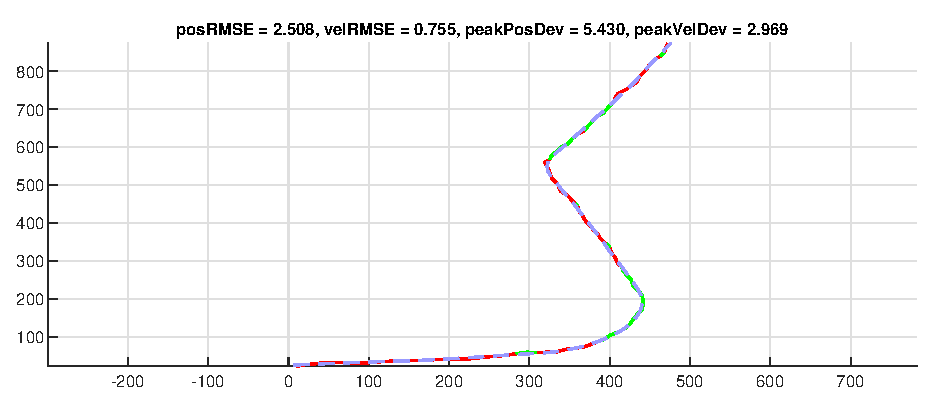
\includegraphics[width=\textwidth]{figures/ga_1/2_estimated_trajectory}
        \caption{Trajectory for simulated data}
        \label{fig:ga_1_2_estimated_trajectory}
    \end{subfigure}%
    ~
    \begin{subfigure}[h]{0.4\textwidth}
        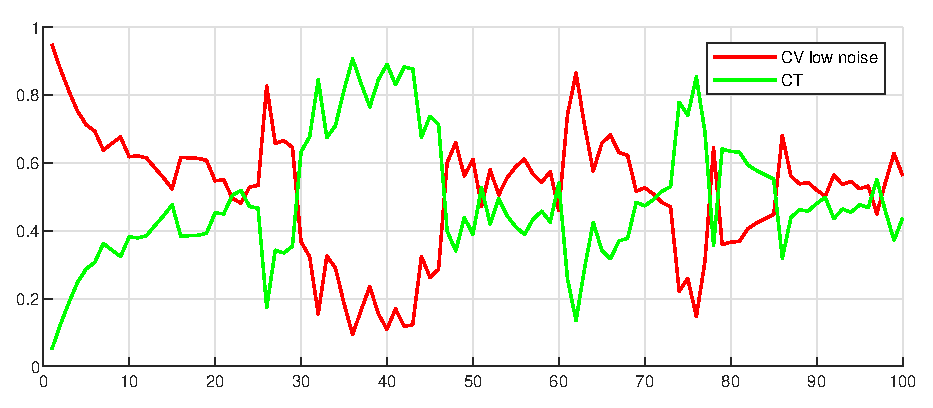
\includegraphics[width=\textwidth]{figures/ga_1/2_probs}
        \caption{Probabilities simulated data}
        \label{fig:ga_1_2_probabilities}
    \end{subfigure}
    \caption{The same colour code was utilised for visualising the active modes in the trajectory as the probability. For the trajectory, ground truth is represented as a dashed line. }
    \label{fig:ga_1_2_traj_and_probs} 
\end{figure}

Finally, for the IMM-PDAF, the clutter rate $\lambda$, detection probability $P_D$ and the validation gate were tuned. The clutter rate was tuned to $\lambda = \SI{1e-4}{}$, and as there were very few false alarms, this could be chosen as a low value. Furthermore, as the only place the clutter rate is used in the IMM-PDAF is to scale the probability of no detection, there was really no use further decreasing $\lambda$, as it already would put the association likelihood ratio for no detection very low. The detection probability is tuned to be rather high, with $P_D = 0.95$, as it is expected that there is a good chance of detection for this data set. A validation gate size of $5^2$ seemed also to give decent results. Increasing it would generally not make the tracker worse overall, but would increase the magnitude of certain errors, which would then spike. Decreasing it would of course make it more difficult for any measurements to be gated, such that this value seemed to be the best compromise between gating all and no measurements. The resulting consistency plot can be seen as \cref{fig:ga_1_2_NEES}, and the average NEES were for position $1.9248$, for velocity $1.1427$ and overall $3.0887$. The errors seem generally ok, and limited in amplitude, as seen from \cref{fig:ga_1_2_error}. 

\begin{figure}[ht]
	\begin{subfigure}[h]{0.4\textwidth}
		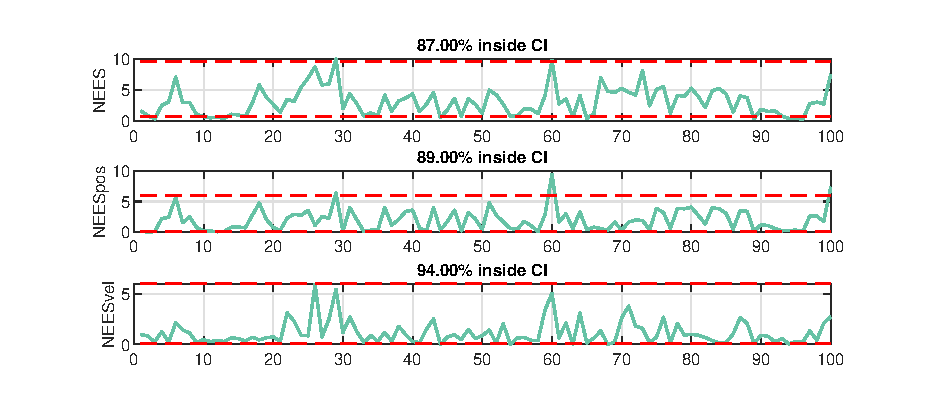
\includegraphics[width=\textwidth]{figures/ga_1/2_NEES}
		\caption{NEES for simulated data}
		\label{fig:ga_1_2_NEES}
    \end{subfigure}% 
    ~
    \begin{subfigure}[h]{0.4\textwidth}
        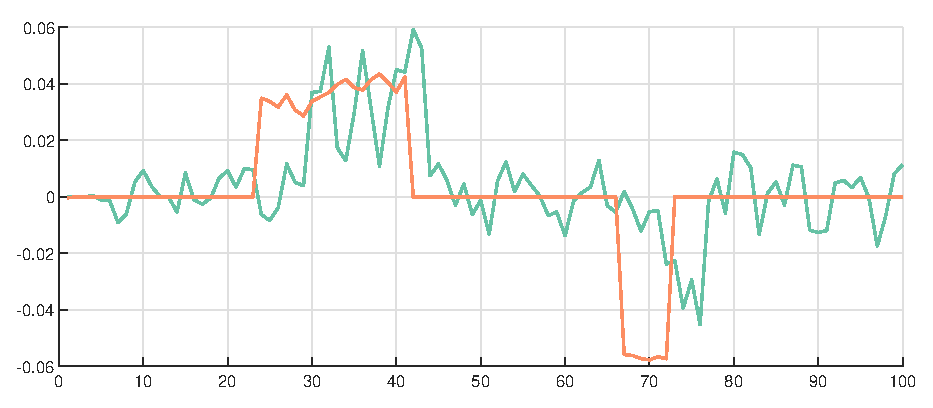
\includegraphics[width=\textwidth]{figures/ga_1/2_error}
        \caption{Errors for simulated data}
        \label{fig:ga_1_2_error}
    \end{subfigure}
    \caption{The NEES and errors from the simulated data. }
    \label{fig:ga_1_2_NEES_and_error} 
\end{figure}

\subsection{IMM-PDAF for joyride data set}
Initially, the IMM-PDAF for the Joyride data set was tuned similarly to the tracker for the simulated data set, and especially for the low noise CV model and the CT model, similar values were used. Furthermore, it should be noted that the Joyride data set also was noisier, such that more lenient tuning was necessary. For this data set, a high noise CV model was also included, which could \textit{take over} if both the low noise CV model and the CT model were uncertain. Otherwise, the overall structure of the tracker is the same as for the simulated data set. 

The measurement noise covariance parameter was again the same for the CT and two CV models, and was set to $25^2$. Though this seemed rather higher than necessary, however lowering it would especially push the positional NEES too high. Similar responses were generated from tuning the acceleration noise covariance parameters and turn-rate noise covariance parameter for the different models. Then, for the low noise CV model, the acceleration noise covariance parameter was tuned to $0.5$, for the high noise CV model, the acceleration noise covariance parameter was tuned to $20$ and for the CT model, the acceleration noise covariance parameter was tuned to $\SI{1e-4}{}$ and the turn-rate noise covariance parameter was tuned to $\SI{2e-4}{}$. Similarly to the results from the simulated data, these models handle their trajectories well, as can be seen from \cref{fig:ga_1_joyride_estimated_trajectory}. 

As for the IMM used in the simulated data set, the transition matrix $\pi$ was tuned to prefer to stay in the CT model, so that the tracker should prefer to continue a turn if it was already turning. Since the high noise CV model was included primarily to handle high noise areas where it could be unambiguous whether to use the low noise CV or CT model, this transition probability was set lower than the others, as those should be preferred. From observing the track and measurements, there also seemed to be unambiguous which of the other modes each should transition to, and as such these transitions were set to be equally likely, see \cref{eq:ga_1_joyride_pi_matrix}. The resulting changes to the probabilities can be seen from \cref{fig:ga_1_joyride_probabilities}. 

\begin{equation}
    \label{eq:ga_1_joyride_pi_matrix}
    \pi = \begin{bmatrix}
        0.900 & 0.025 & 0.075 \\
        0.050 & 0.950 & 0.075 \\
        0.050 & 0.025 & 0.850 
    \end{bmatrix}
\end{equation}

\begin{figure}[ht]
    \begin{subfigure}[h]{0.4\textwidth}
        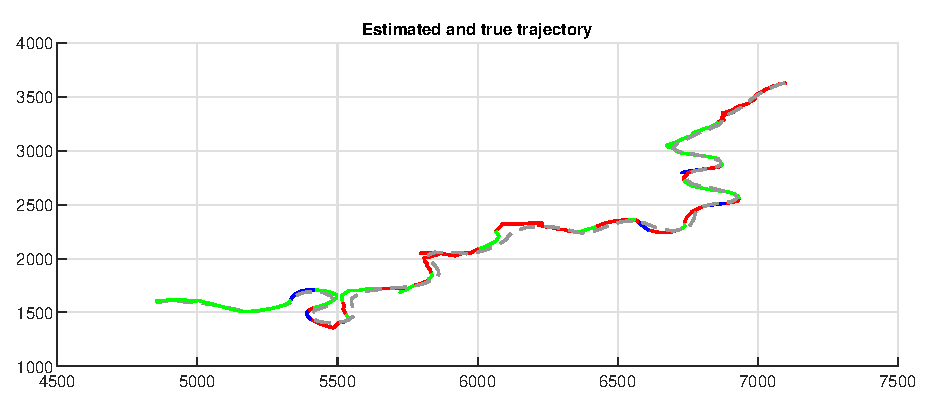
\includegraphics[width=\textwidth]{figures/ga_1/joyride_estimated_trajectory}
        \caption{Trajectory for joyride data}
        \label{fig:ga_1_joyride_estimated_trajectory}
    \end{subfigure}%
    ~
    \begin{subfigure}[h]{0.4\textwidth}
        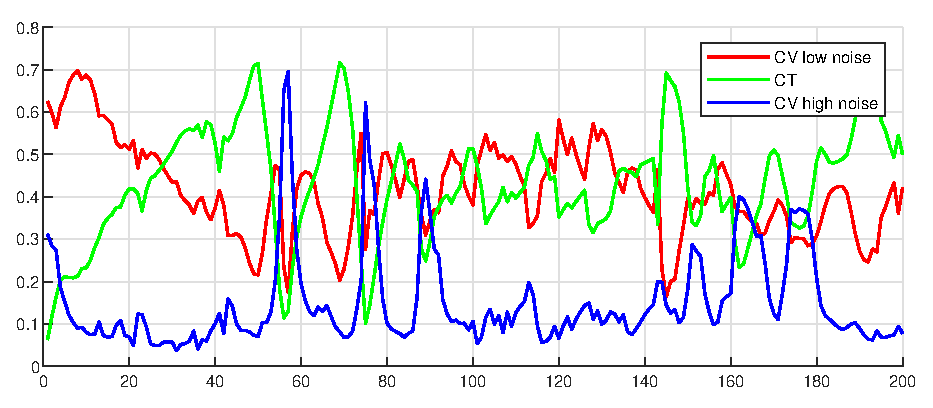
\includegraphics[width=\textwidth]{figures/ga_1/joyride_probs}
        \caption{Probabilities joyride data}
        \label{fig:ga_1_joyride_probabilities}
    \end{subfigure}
    \caption{The same colour code was utilised for visualising the active modes in the trajectory as the probability. For the trajectory, ground truth is represented as a dashed line. }
    \label{fig:ga_1_joyride_traj_and_probs} 
\end{figure}

The IMM-PDAF was tuned to have a lower clutter rate and higher detection probability than for the simulated data, while keeping the gate size. The clutter rate was tuned to be $\lambda = \SI{5e-5}{}$. Higher values would inevitably make the tracker loose track and converge to one mode, rendering the tracker useless. As the clutter rate affects the likelihood ratio for no detection, a higher clutter rate implies a higher likelihood compared to a lower clutter rate, and a higher value would be given to the association probability for no detection. The detection probability was tuned to $P_D = 0.97$, which is a rather high value. It was possible to reduce $P_D$ and, specifically, improve the percentage where the NEES is inside CI, but at a cost of the NEES for the velocity, and a higher $P_D$ was chosen so that the NEESes would be more similar. 

The resulting consistency plot can be seen \cref{fig:ga_1_joyride_NEES}, and the average NEESes were found as $1.6653$ for position, $1.3966$ for velocity and $3.4346$ overall. Both the plots and the averages tend to be closer to the lower bound of the confidence interval, though as can be noted, there were certain spikes in the plot. These were difficult to handle as they seemed to originate from especially bad measurements, and a compromise was made where the consistency would tend to be low, in exchange for limiting the spikes. The errors also seemed to be acceptable, see \cref{fig:ga_1_joyride_error}. 

\begin{figure}[ht]
	\begin{subfigure}[h]{0.4\textwidth}
		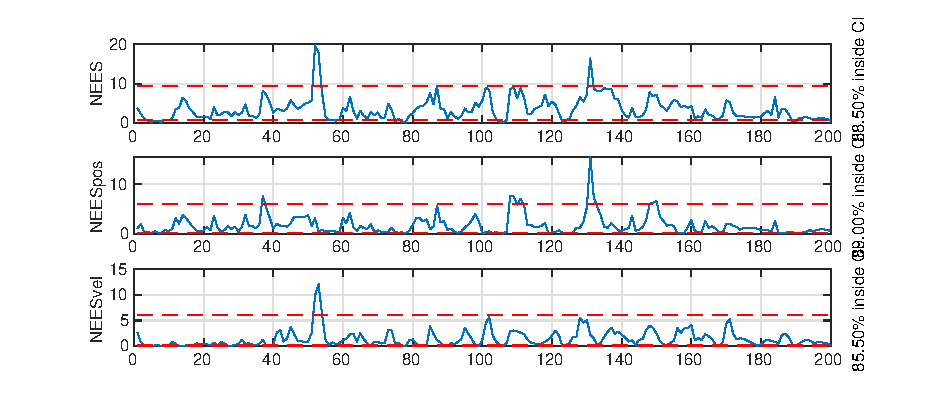
\includegraphics[width=\textwidth]{figures/ga_1/joyride_NEES}
		\caption{NEES for joyride data}
		\label{fig:ga_1_joyride_NEES}
    \end{subfigure}% 
    ~
    \begin{subfigure}[h]{0.4\textwidth}
        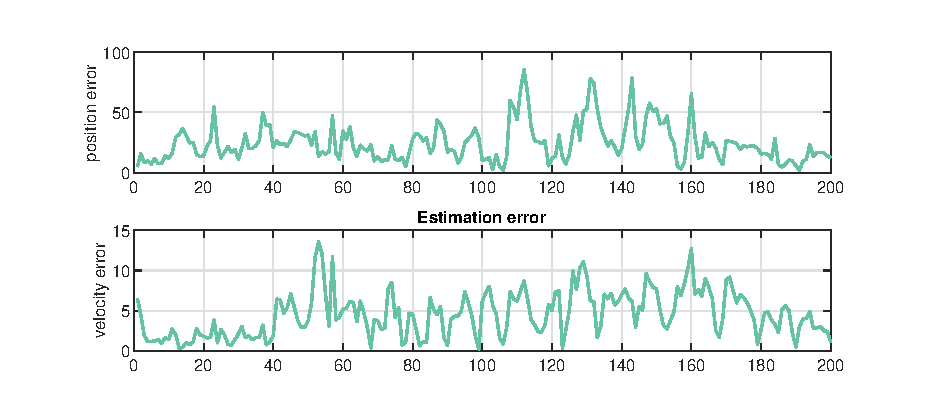
\includegraphics[width=\textwidth]{figures/ga_1/joyride_error}
        \caption{Errors for joyride data}
        \label{fig:ga_1_joyride_error}
    \end{subfigure}
    \caption{The NEES and errors from the joyride data. }
    \label{fig:ga_1_joyride_NEES_and_error} 
\end{figure}

% stepsWithClose =
%    136
% meanMeasError =
%     3.6865
%    -7.2491
% covMeasError =
%   119.3970   14.9059
%    14.9059  116.2221
% stds =
%    10.9269
%    10.7806
% covEllSize =
%    10.1400
%    11.5239
% meanMinMeasDists =
%   300.0264
% meanNumberOfCloseMeasurements =
%     0.6800
% CI2K =
%     1.7324    2.2865
% ANEESpos =
%     1.6653
% ANEESvel =
%     1.3966
% CI4K =
%     3.6176    4.4014
% ANEES =
%     3.4346

% note that q lower for CT? 

% parameters 

% In the report you should do a bit more analysis of what happens with different parameters settings, and base your choice on relevant plots and numbers. To achieve a full score we also want to see at least some minor reflections on the algorithm and the approximations it does in light of your results. 
% We want to see an analysis of what happens and why with some different parameter/model settings, and base your choice of model and parameters on relevant plots and numbers. To achieve a full score we also want to see at least some minor reflections on the algorithm and the approximations it does, in light of your results. Relating results in this tasks or assignments to the previous task can give additional points. 

% \begin{figure}[ht]
% 	\begin{subfigure}[h]{0.4\textwidth}
% 		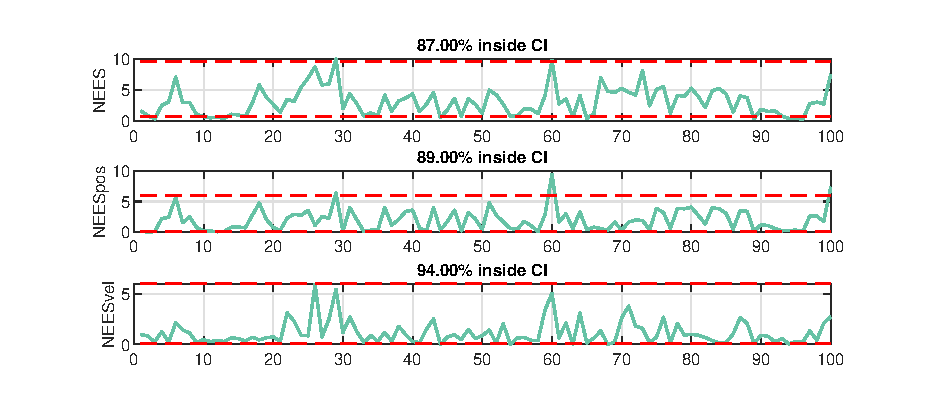
\includegraphics[width=\textwidth]{figures/ga_1/2_NEES}
% 		\caption{NEES for simulated data}
% 		\label{fig:ga_1_2_NEES}
%     \end{subfigure}%
%     ~
% 	\begin{subfigure}[h]{0.4\textwidth}
% 		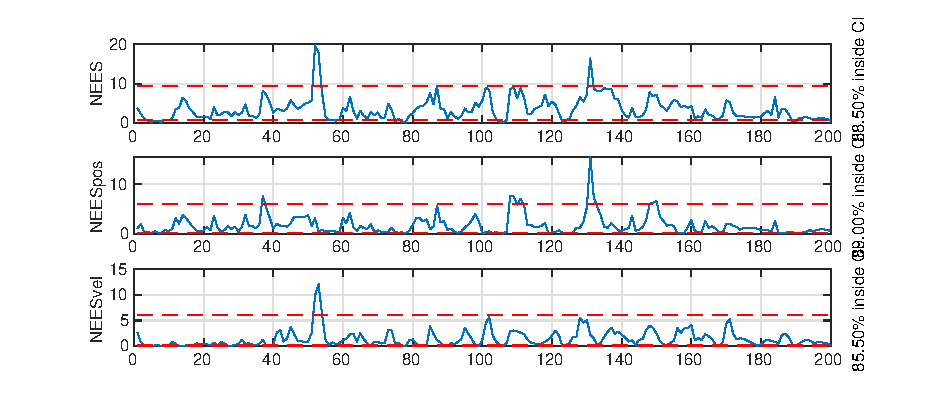
\includegraphics[width=\textwidth]{figures/ga_1/joyride_NEES}
% 		\caption{NEES for Joyride}
% 		\label{fig:ga_1_joyride_NEES}
% 	\end{subfigure}
%         \\
%     \begin{subfigure}[h]{0.4\textwidth}
%         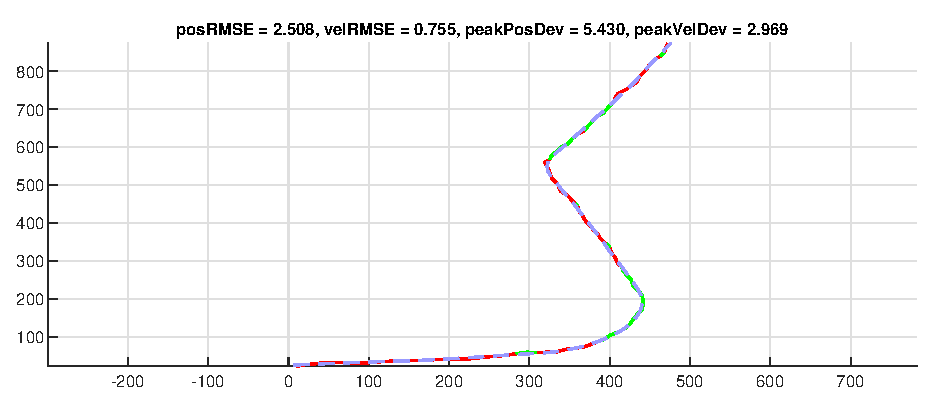
\includegraphics[width=\textwidth]{figures/ga_1/2_estimated_trajectory}
%         \caption{Trajectory for simulated data}
%         \label{fig:ga_1_2_estimated_trajectory}
%     \end{subfigure}%
%     ~
%     \begin{subfigure}[h]{0.4\textwidth}
%         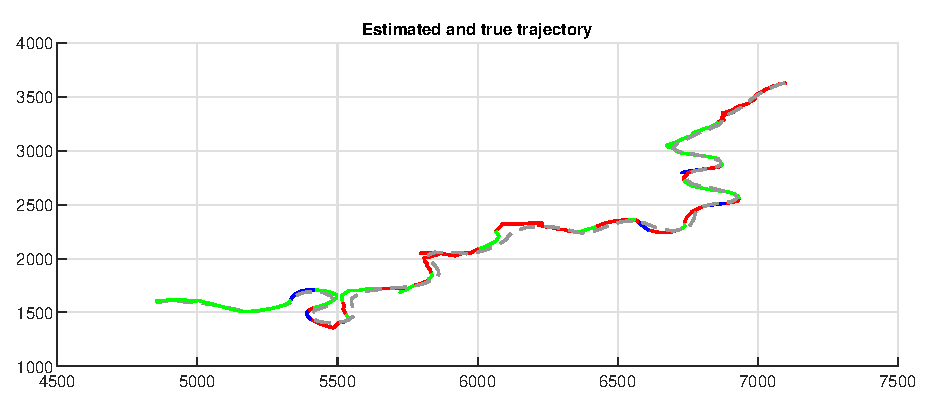
\includegraphics[width=\textwidth]{figures/ga_1/joyride_estimated_trajectory}
%         \caption{Trajectory for Joyride}
%         \label{fig:ga_1_joyride_estimated_trajectory}
%     \end{subfigure}
%         \\
%     \begin{subfigure}[h]{0.4\textwidth}
%         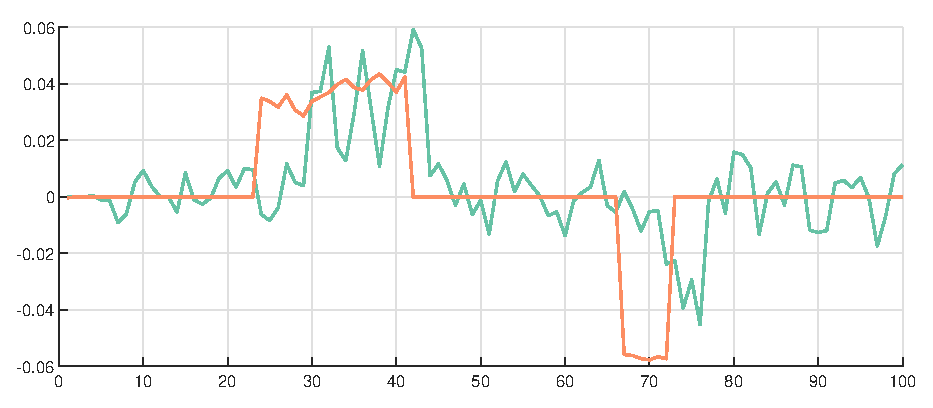
\includegraphics[width=\textwidth]{figures/ga_1/2_error}
%         \caption{Errors for simulated data}
%         \label{fig:ga_1_2_error}
%     \end{subfigure}%
%     ~
%     \begin{subfigure}[h]{0.4\textwidth}
%         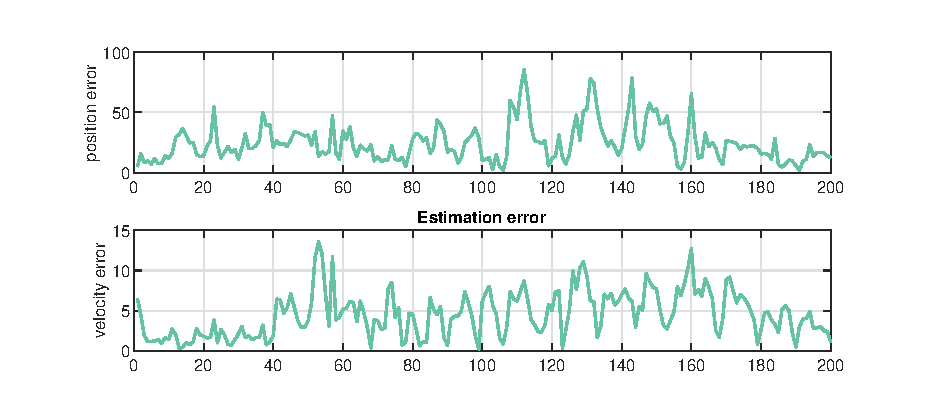
\includegraphics[width=\textwidth]{figures/ga_1/joyride_error}
%         \caption{Errors for Joyride}
%         \label{fig:ga_1_joyride_error}
%     \end{subfigure}
%         \\
%     \begin{subfigure}[h]{0.4\textwidth}
%         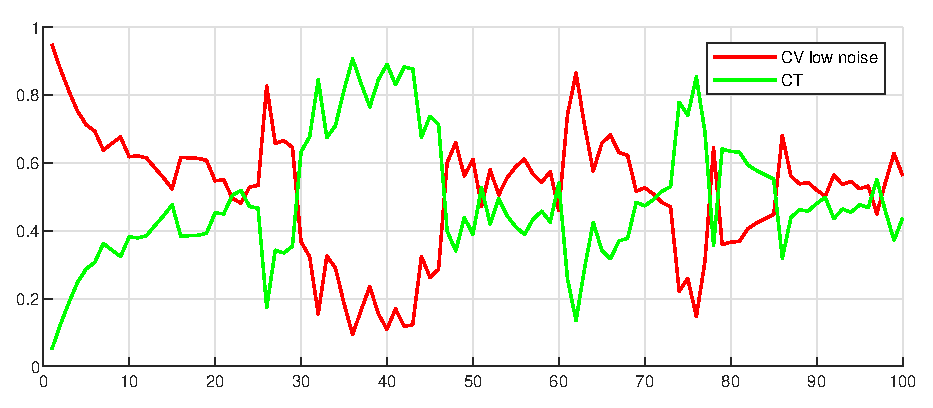
\includegraphics[width=\textwidth]{figures/ga_1/2_probs}
%         \caption{Probabilities simulated data}
%         \label{fig:ga_1_2_probabilities}
%     \end{subfigure}%
%     ~
%     \begin{subfigure}[h]{0.4\textwidth}
%         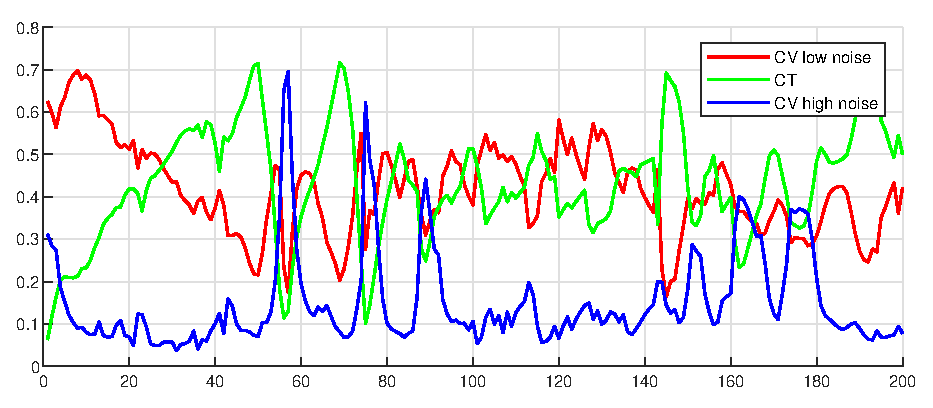
\includegraphics[width=\textwidth]{figures/ga_1/joyride_probs}
%         \caption{Probabilities for Joyride}
%         \label{fig:ga_1_joyride_probabilities}
%     \end{subfigure}
%     \caption{The same colour code was utilised for visualising the active modes in the trajectories as the probabilities. For the trajectories, ground truth is represented as a dashed line. }
%     \label{fig:ga_1} 
% \end{figure}

\subsection{IMM-PDAF discussion}
The IMM-PDAF works under the single-target assumptions, as seen from \cite[p. 105]{Edmund}, which all seem reasonable considering both the simulated and real data sets. In the simulated data set, there is initially good reason to suspect that these assumptions were considered when the data set was generated, and it may therefore be more interesting to consider the real data set. There are a smaller number of measurements for each time step than there seemed to be for the simulated data set, and therefore, it may seem like the job of the tracker for this data set is, primarily, to consider whether there is a detection or not. In certain cases, the measurements are also pretty far away from each other and the track, which could also make it easier for the tracker. Since it is likely that several raw measurements may originate from the sensor, like a RADAR, it is common to apply some form of clustering to reduce the measurements from the target to one single measurement, see \cref{fig:ga_1_joyride_measurements_and_estimated_trajectory} to see the joyride measurements used. Depending on the method for clustering, this is very likely to make the tracker work, and it is computationally a good idea to use the single target assumption, though this clustering may also cluster bad measurements as well, which may make the tracking more difficult. This was not further explored here, as there doesn't seem to be a need for it. 

% IMM-PDAF
There are certain simplifications done in this algorithm to make it more viable, and as mentioned above, assuming that only one measurement may originate from the target allows for a more computationally efficient algorithm. Additionally, as the associations (and modes) are seen as mixtures, then as to not end up with an extremely large number of values, the mixtures can be reduced by moment matching. This also makes the tracker a more computationally efficient algorithm, and keeps the memory usage manageable. 

% gate
    % at least one is gated
Gating of the measurements, is done, for each measurement, by checking the NISes for all modes given this measurement. If a measurement is gated for one mode, it is gated for all modes. This assumption seems to be good, as it then seems like at least one of the models can \textit{accept} this measurement. There may still be cases where a stricter gating rule could have been considered, like only applying the measurements to the specific modes with NISes within the gate size. For these data sets however, there haven't been any specific cases where this assumption has caused problems. 

\begin{figure}[ht]
    \centering
    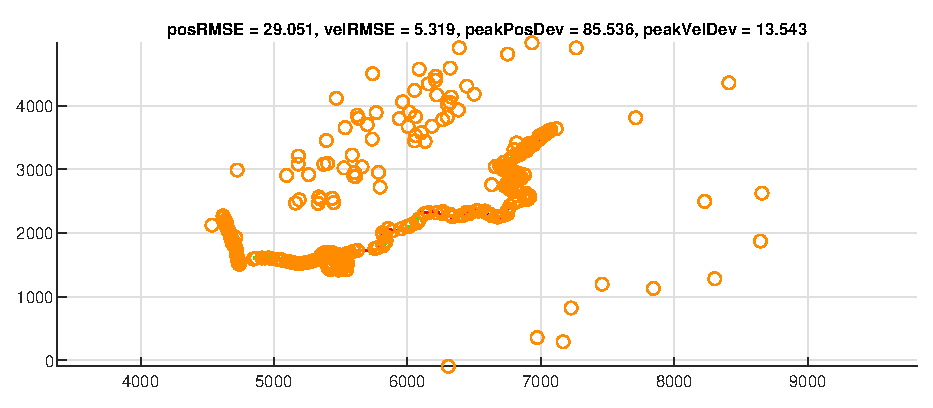
\includegraphics[width=0.5\textwidth]{figures/ga_1/joyride_measurements_and_estimated_trajectory} 
    \caption{Measurements and estimated trajectory for the joyride data set. }
    \label{fig:ga_1_joyride_measurements_and_estimated_trajectory}
\end{figure}

% IMM
% Certain simplifications were also made to make the code easier to implement, which probably slows the tracker slightly down, as when calculating the log-likelihood ratios, the \textit{update}-method from the IMM was utilised, and most of the results were discarded. If there was a need to save a small amount of time, or reduce the number of operations done, there are some places in the code where one could save time. This could be necessary if there was a need to run the tracker online. 

% EKF
Using the EKF, with the CV and CT models, is also a simplification, especially for the joyride data set. For the simulated data set, these models were probably used to generate the data set. It should therefore be possible to get very good result using these models, as seen from \cref{fig:ga_1_2_estimated_trajectory}. The joyride data set, however, is different, as there is not \textit{really} an underlying model which generated this data set. Still, by using several simpler models, including a high-noise mode for robustness, decent tracking was achieved for the joyride data set as well, as can be seen from \cref{fig:ga_1_joyride_estimated_trajectory}. 

% task 2 and 3
    % NEES with confidence bounds
        % total
        % position
        % velocity
    % estimation error (Euclidian distance)
        % position 
        % velocity
    % averaged NEESes 
    % number of times the NEESes fall within the confidence region
    % position and velocity RMSE (mean taken over time)

% parameters based on this
% other plots




% For task 2 and 3, we want to see a plot of the total, position and velocity NEES along with your chosen confidence bounds for these, and estimation error (Euclidian distance) in position and velocity for the tracker run with your chosen parameters. 
% In addition we want the numbers of the averaged NEESes along with their confidence bounds, the number of times the NEESes fall within the confidence regions and the positional and velocity RMSE (mean taken over time). 
% We then expect you to base your choice of parameters on these values, and compare to other sets of parameters. 
% To show plots of other parameter settings is up to you. 
\section{Graded Assignment 2}\label{sec:graded_assignment_2}

% A full answer and result analysis is expected for task 3 and 4. For task 3 you should include a plot of the different states over time as well as the error states for your choice of parameters, in addition to NEES and NIS over time for the same set of parameters. In task 4 the same plots are expected, of course excluding anything that needs the ground truth. For both tasks it should be made clear why the parameters were chosen in terms of error metrics, consistency and overall result. Answers and analysis should connect theory and results to the real world, and show your understanding for the problem and solution. Try to connect the reuslts on the simulated data to the results of the real data where it is possible. 

An error-state Kalman filter (ESKF) for a GNSS-aided fixed-wing UAV was implemented in MATLAB. The implementation is based on the standard formulation in \cite{Sola}. But most notably, IMU sensor correction matrices has been added to counteract any mounting errors, scaling errors and orthogonality errors in the accelerometer and rate gyro. Furthermore, leverarm componsation for the GNSS receiver is also implemented.

\subsection{INS for simulated fixed-wing UAV}

%Tuning values, how we tuned (NIS, NEES, RMSE, want bias to converge somewhat, not wander, commen sense)

%Heading observability - heading error large, spikes?? Probably low when turning, then larger when straight/no acceleration. Also see this in attitude NEES compared to others.

%Misalignment matrix

% discuss bias models

The ESKF was first tuned to a simulated dataset. The GNSS measurement standard deviation was tuned to $0.4$ in each degree of freedom. The measurement noise covariance is therefore $R=0.16 I ^2$. For the accelerometer the measurement noise covariance and bias driving noise covariance was tuned to be $q_{a} = (\SI{4e-2})^2$ and $ q_{ab} = (\SI{1e-3})^2$ respectively. Similarily for the rate gyro the measurement noise covariance and bias driving noise covariance was tuned to be $q_{\omega} = (\SI{8e-4})^2$ and $q_{\omega b} = (\SI{1e-6})^2$ respectively. Finally the time constants in the Gauss-Markov bias processes were both tuned to be $T_b = \SI{1e8}{s}$.

Firstly, the tuning was based on common sense. For instance the GNSS measurement covariance was initially based on a reasonable guess from a physical perspective and then more thoroughly tuned. This more thorough tuning was based on calculating and plotting the errors in position, velocity, attitude and bias. Furthermore the corresponding NEES in position, velocity, attitude and biases, as well as the overall NEES and NIS was calculated and analysed during the tuning process. 

The resulting position estimate is plotted in \cref{fig:ga_2_sim_trajectory}, the state and state errors are presented in \cref{fig:ga_2_sim_state} and \cref{fig:ga_2_sim_errors} and finally the consistency analysis is presented in \cref{fig:ga_2_sim_consistency}. Note that the consistency figures are presented in logarithmic scale. Furthermore, the average NEES and NIS is approximately 18.57 and 2.27 respectively.

\begin{figure}[ht]
    \centering
	\begin{subfigure}[b]{0.45\textwidth}
		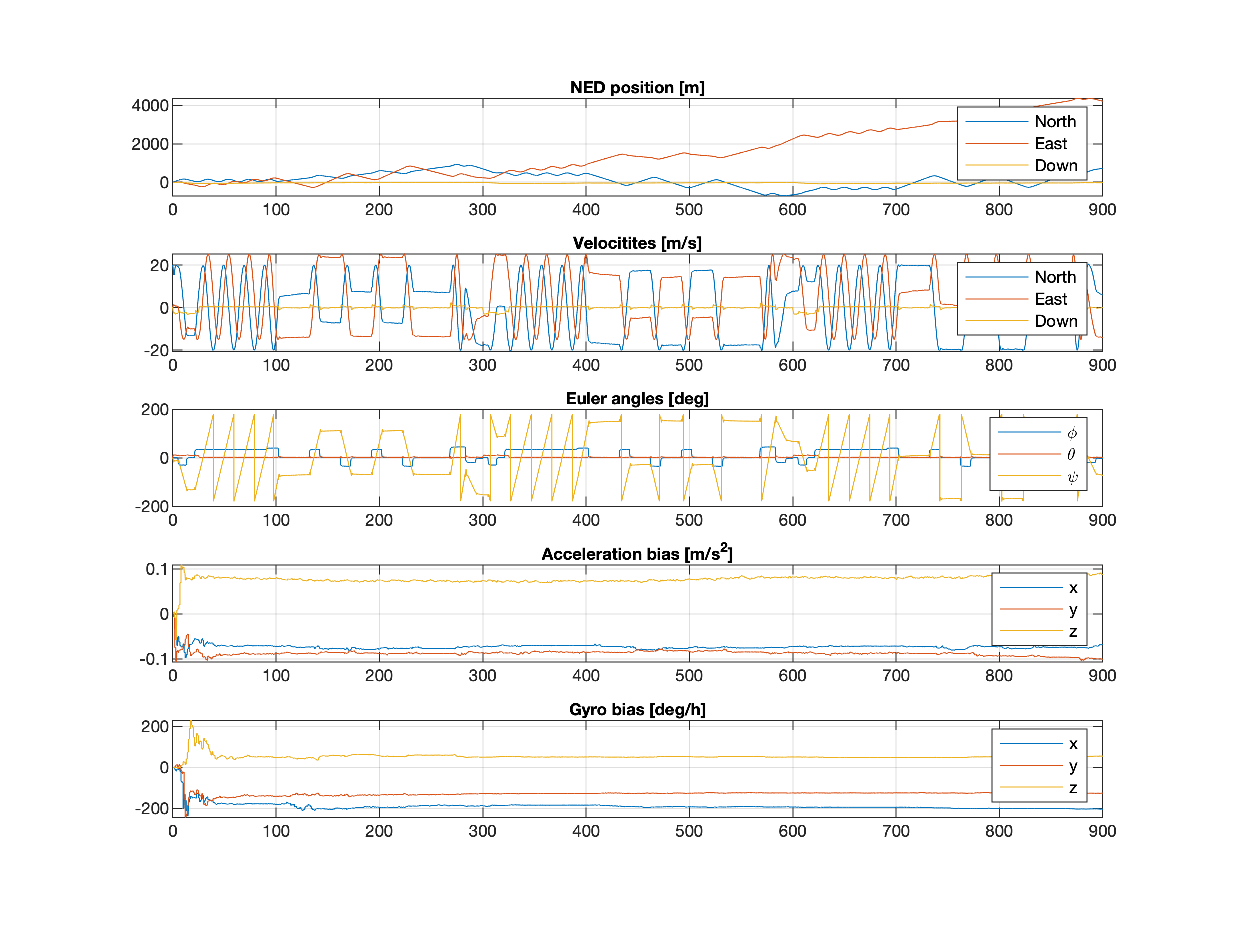
\includegraphics[width=\textwidth]{figures/ga_2/sim_state}
		\caption{UAV ESKF states}
		\label{fig:ga_2_sim_state}
	\end{subfigure}%
       ~
	\begin{subfigure}[b]{0.45\textwidth}
		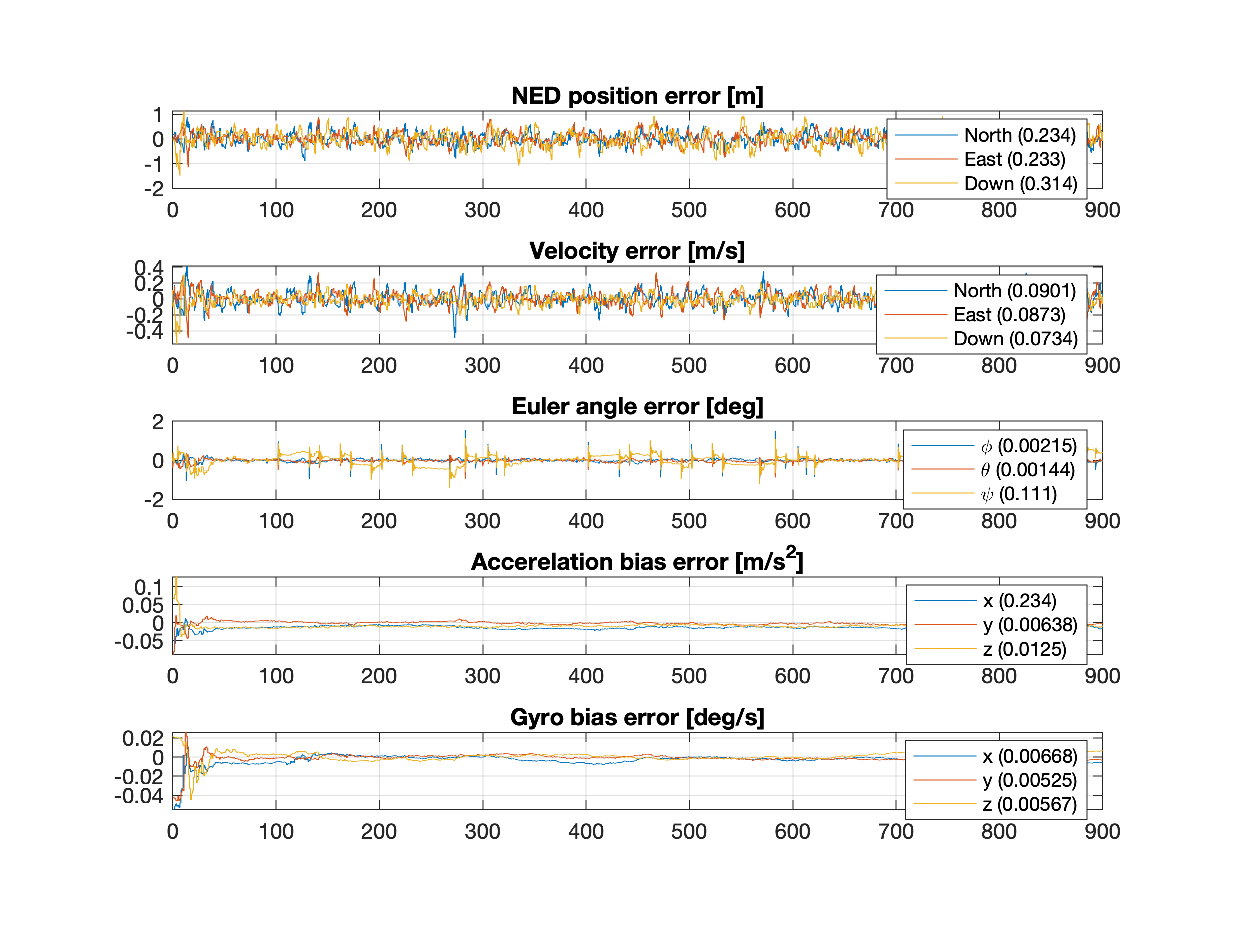
\includegraphics[width=\textwidth]{figures/ga_2/sim_errors}
		\caption{UAV ESKF state errors}
		\label{fig:ga_2_sim_errors}
	\end{subfigure}
    \label{fig:ga_2_sim_state_errors} 
\end{figure}

\begin{figure}[ht]
    \centering
	\begin{subfigure}[b]{0.45\textwidth}
		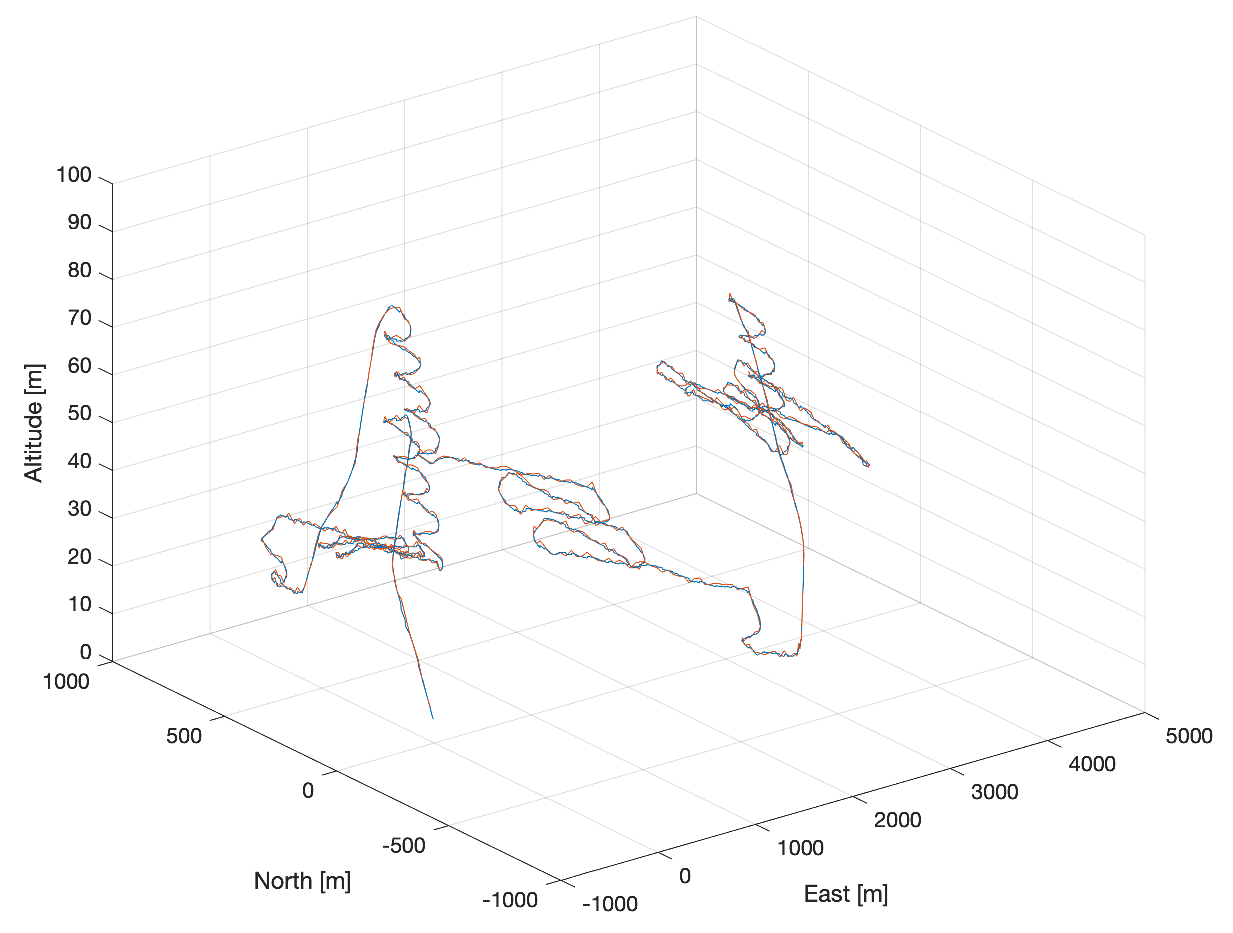
\includegraphics[width=\textwidth]{figures/ga_2/sim_trajectory.eps}
    \caption{Estimated UAV trajectory}
    \label{fig:ga_2_sim_trajectory}
	\end{subfigure}%
       ~
	\begin{subfigure}[b]{0.45\textwidth}
		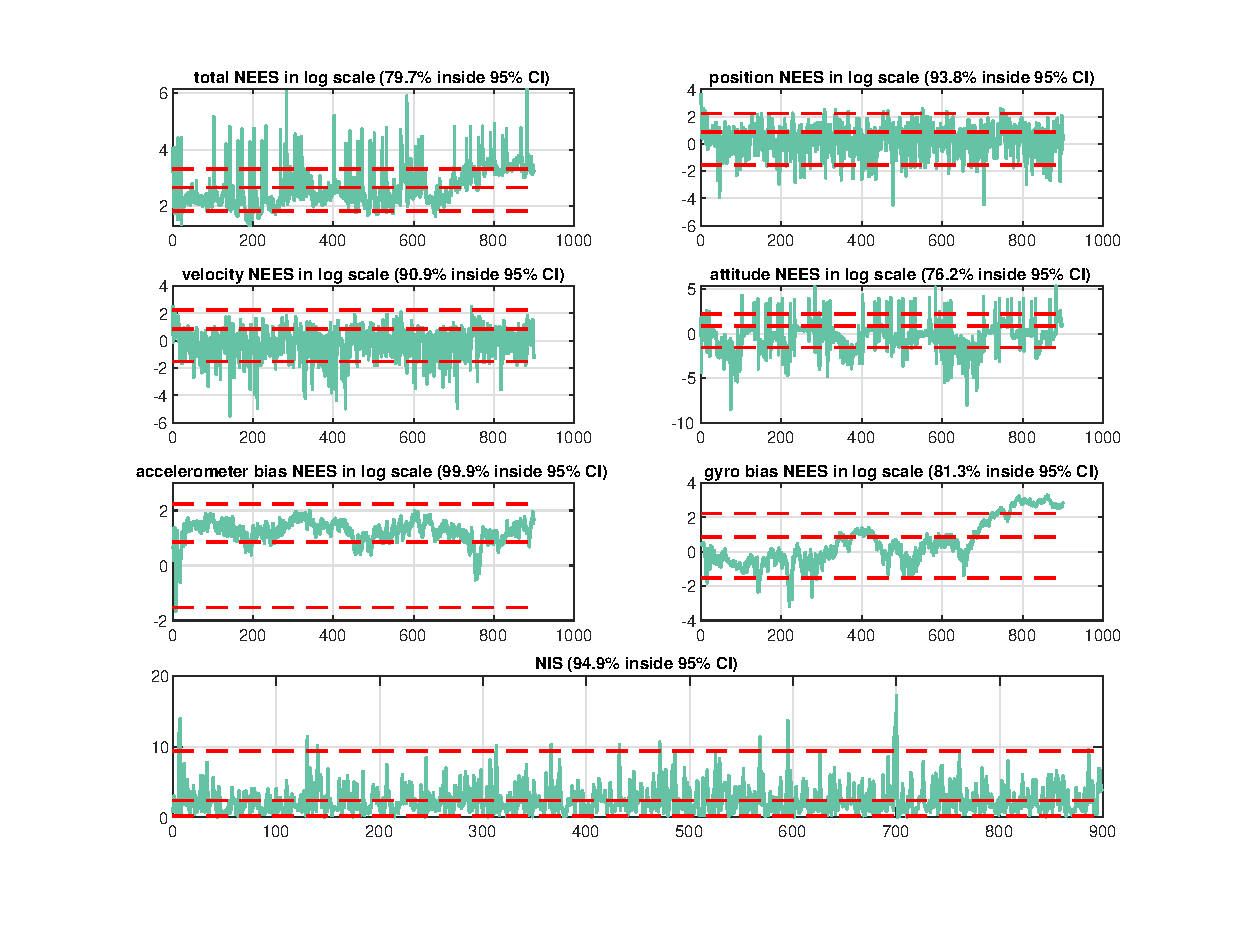
\includegraphics[width=\textwidth]{figures/ga_2/sim_consistency.eps}
    \caption{UAV ESKF consistency analysis}
    \label{fig:ga_2_sim_consistency}
	\end{subfigure}
    \label{fig:ga_2_sim_trajectory_consistency} 
\end{figure}

The ESKF was in particular tuned such that the bias states converged nicely, such that the errors propagated in the system from sensor drift were minimised. It should be emphasised that one of the main features that makes the ESKF robust is the IMU bias estimation, and it was therefore also emphasised in the tuning process.

The consistency was also emphasised when tuning the ESKF. We see from \cref{fig:ga_2_sim_consistency} that most of the different normalized square errors are all in the 80\% or 90\% range inside the calculated confidence intervals, which was found to be satisfactory. One should especially note that the attitude NEES is only about 76\% inside the confidence interval. Studying the heading error in \cref{fig:ga_2_sim_errors} can give some insight into why this might be the lowest NEES. It is observed that the heading is at certain time intervals far off the ground truth, which is also confirmed by the RMSE of 0.111. This is about two magnitudes higher error than for pitch and roll. This is caused by the fact that pitch and roll are directly observable from the gravitational force acting on the accelerometer. Heading, on the other hand, is only observable when the system is exited by a manoeuvre. The heading error, therefore, has certain sections where it is unobservable and the update step is not able to correct the constant offset from the true value. This is further supported by studying the time intervals when the UAV is doing a spiral manoeuvre e.g. from about 300 to 400 seconds or from 600 to 700 seconds. In these intervals the heading is observable and as a consequence, we observe that the error drops to the same magnitude as the pitch and roll, before it starts acting unexpectedly again when the UAV starts flying straight. This issue might be why both the attitude NEES and total NEES is somewhat worse than the others. So the heading estimation would therefore not work if the UAV was standing still. 

When letting the sensor correction matrices be identity matrices, and thereby removing any sensor correction, the ESKF estimation performance is noticeably worse. While the filter is still able to reliably estimative velocity and position with the aid of the GNSS, the estimates of heading and sensor biases are much worse. Most importantly, the rate gyro and accelerometer biases no longer converge to the true sensor biases. This means we are not able to remove the bias in the measurements, and as a consequence, they are integrated and propagated through the Kalman filter. This makes all the RMSEs significantly worse, and especially the heading now drifts quickly when the UAV is not turning.

Then the NEES and NIS naturally also worsens significantly. While the position and velocity NEES is still somewhat within the confidence intervals at 85.2\% and 64.9\% respectively, the attitude, accelerometer bias and gyro bias is at 3.09\%, 14.6\% and 2.89\% respectively. This further supports the claim above about how important IMU bias compensation is when trying to design a robust attitude estimator. It is then evident that correction for sensor misalignment, scaling errors and orthogonality errors are a critical part of designing such an estimator. Neglecting the GNSS lever arm, on the other hand, has no noticeable effect on the estimator performance.

Finally, it must be said that finding the sensor correction matrices is not trivial, and the results will be empirically based and not absolutely correct. Therefore we will always have some sensor misalignment and miss-scaling in a physical system, especially since these matrices will, in reality, be time-varying.

\subsection{INS for real fixed-wing UAV}

% tuning a lot the same, but we started by looking at datasheet + simulated values. No NEES now, only NIS. Used GNSS accuracy thing. 

The ESKF was then tuned to a real dataset from a fixed-wing UAV flight. The sensors onboard was a STIM300 IMU and an u-blox M8 GNSS receiver. The GNSS receiver produces an accuracy estimate in standard deviation while operating. This was scaled by a gain parameter, squared and used as a time-varying GNSS measurement noise covariance signal. The gain was tuned to be $k_x = 0.5$.

The IMU measurement noise covariances and bias driving noise covariances were tuned from the Allan variances in the STIM300 datasheet \cite{stim300}. Specifically, the gyro noise and bias noise root Allan variance is \SI{0.15}{\deg\per\sqrt\hour} and \SI{0.5}{\deg\per\hour} respectively. The accelerometer noise and bias noise root Allan variance is \SI{0.06}{\meter\per\second\sqrt\hour} and \SI{0.05}{\meter g} respectively. These values were scaled to the correct units and used as initial parameters in the ESKF. The values were then tuned such that a satisfactory estimate and NIS were produced. The final tuning parameters were 
then $q_{a} = (\SI{9.8e-4})^2$, $ q_{ab} = (\SI{4.9e-4})^2$, $q_{\omega} = (\SI{4.9e-6})^2$ and $q_{\omega b} = (\SI{2.4e-6})^2$. When comparing to the simulated case, one sees that the bias noise standard deviations are of about the same magnitude, while the measurement noise standard deviations are about two magnitudes larger in the simulated case.

The resulting UAV trajectory estimate is presented in \cref{fig:ga_2_real_trajectory} and the estimated states are presented in \cref{fig:ga_2_real_state}. Finally the NIS is presented in \cref{fig:ga_2_real_consistency}. The average NIS was approximately 3.01. Note that since this is a real dataset, we do no longer have the ground truth, and can therefore not calculate the estimation errors and NEES. This certainly makes tuning more challenging, even though access to the IMU datasheet is useful. This shows how it is often helpful to test filter implementations on simulated data first, as has been done in all of the assignments discussed in this report. The Gauss-Markov bias time constants were both tuned to $T_b = \SI{1e16}{s}$, effectively making the bias processes random walks processes.

\begin{figure}[ht]
    \centering
    \begin{subfigure}[b]{0.45\textwidth}
		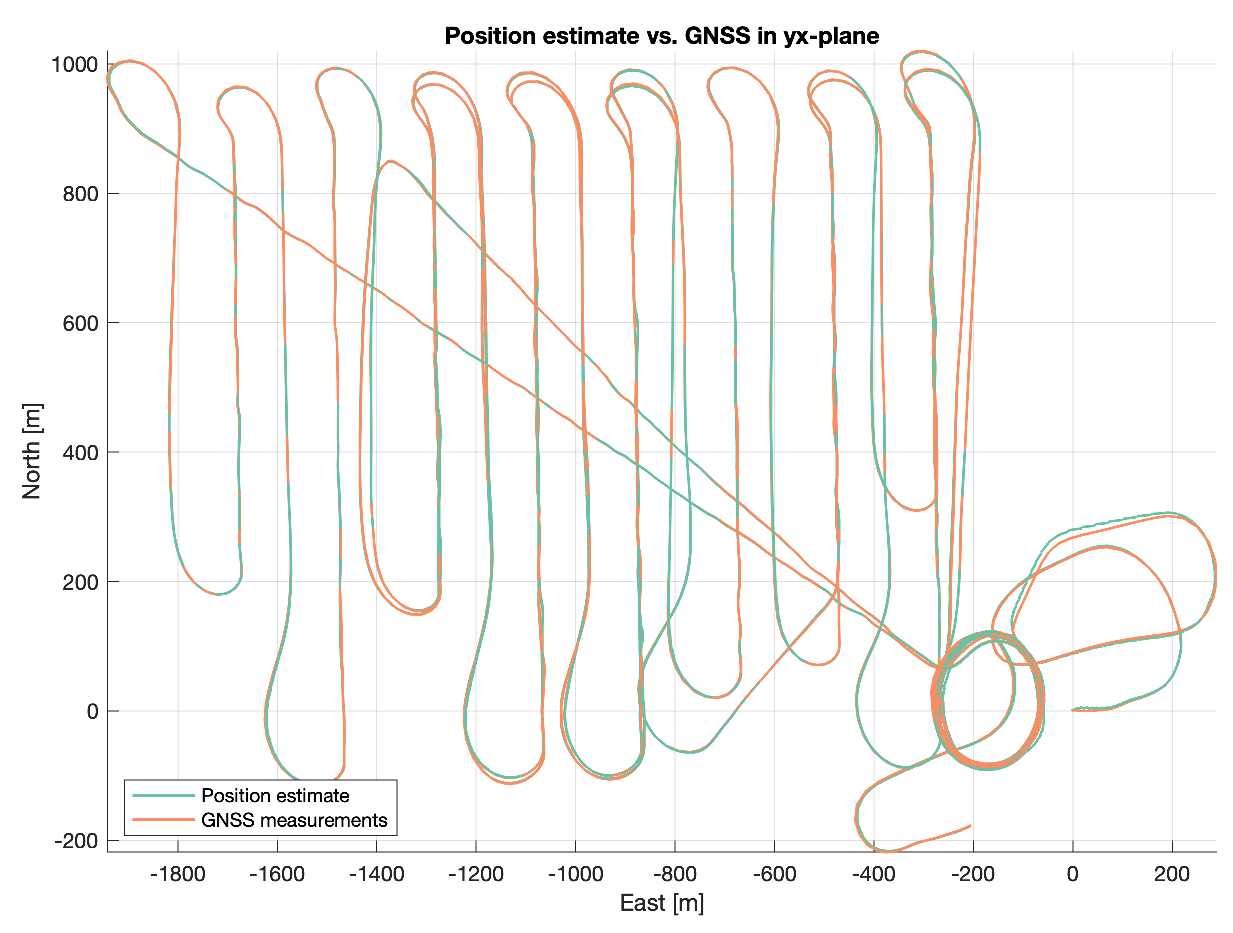
\includegraphics[width=\textwidth]{figures/ga_2/real_trajectory.eps}
        \caption{Estimated UAV trajectory}
        \label{fig:ga_2_real_trajectory}
	\end{subfigure}%
    \begin{subfigure}[b]{0.45\textwidth}
		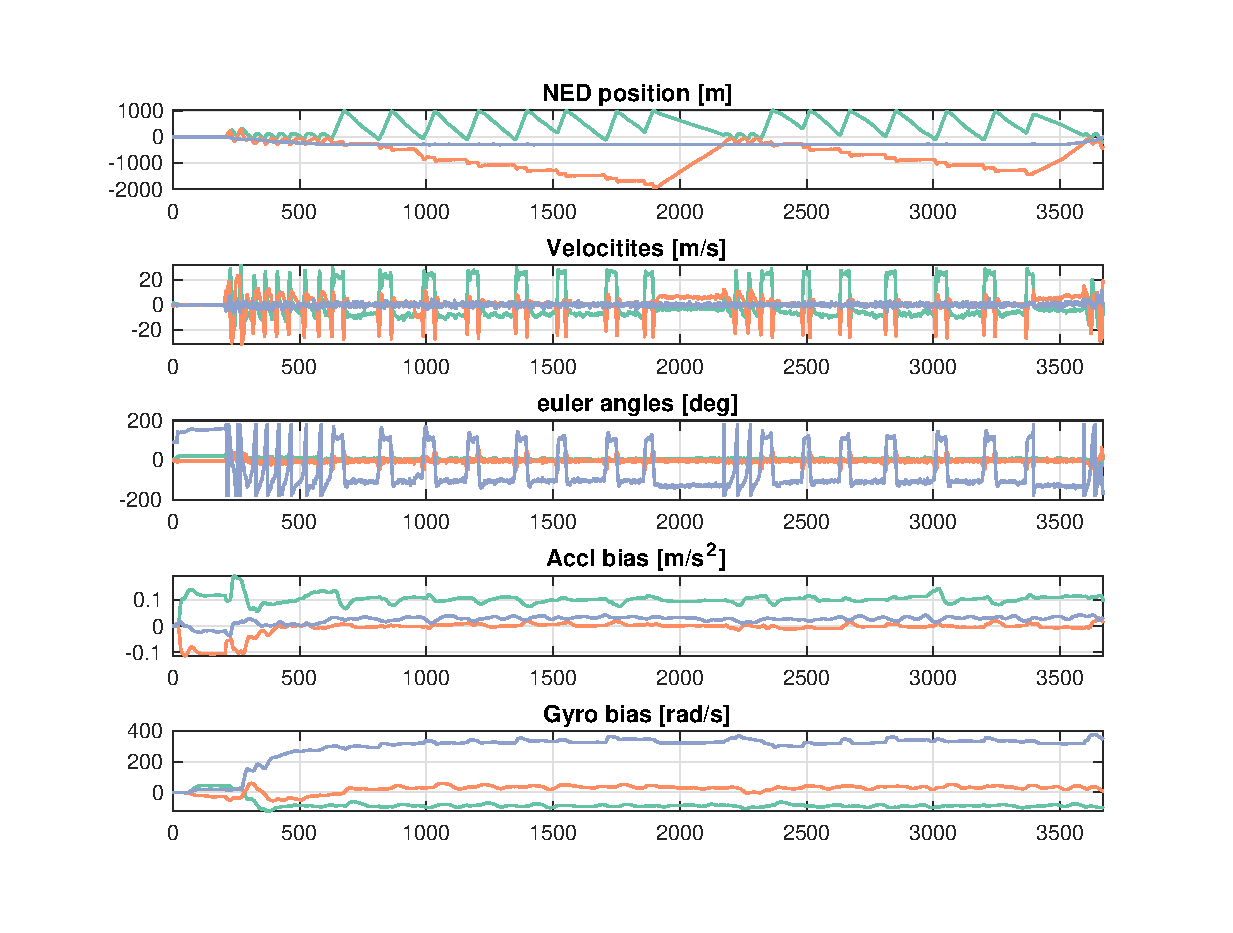
\includegraphics[width=\textwidth]{figures/ga_2/real_state.eps}
        \caption{UAV ESKF states}
        \label{fig:ga_2_real_state}
	\end{subfigure}
    \label{fig:ga_2_real_trajectory_state}
\end{figure}

\begin{figure}[!htb]
    \centering
    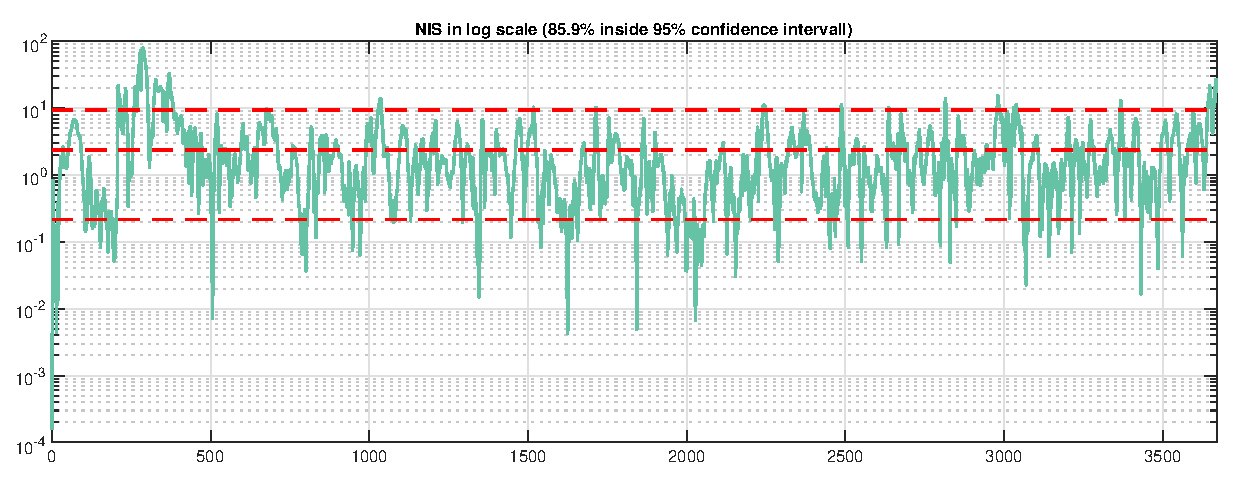
\includegraphics[width=0.8\linewidth]{figures/ga_2/real_consistency.eps}
    \caption{UAV GNSS logarithmic NIS}
    \label{fig:ga_2_real_consistency}
\end{figure}

We observe how the estimated trajectory fits nicely with the GNSS data as one would expect. The estimates are also nicely behaved, while the state trajectories are naturally a lot less smooth in this case compared to the simulation, which is to be expected. In particular, the biases converge over time, with some corrections throughout the flight when the UAV turns and the system is excited. From the heading plot it seems like the bias estimates work well, as there is no noticeable drift in heading. For most of the flight, we see that the heading changes between two almost constant values. This is reflected by the UAV manoeuvres in \cref{fig:ga_2_real_trajectory}, where the UAV flies straight north, then quickly does a U-turn, then flies straight south, then does a U-turn and so on. 

When the sensor correction matrices were set to identity for the real data, it was observed again that thanks to the GNSS measurements the position and velocity estimates are still viable. But the biases do not converge to the same values as before. Interestingly, the heading quickly becomes the opposite of what it was before, and the roll and pitch estimates "switch places", as can be seen in \cref{fig}. This is due to the fact that the sensor frame is no longer approximately aligned with the body frame. While in the simulated case the sensor correction matrices were close to identity, for this data set they are
\begin{equation}
    S_g = \begin{bmatrix}
        -0.0243 & 0.9981  & 0.0454 \\
        -0.9998 & -0.0242 & -0.0255 \\
        -0.0272 & -0.0532 & 0.9949
    \end{bmatrix}, \quad
    S_a = \begin{bmatrix}
        -0.0503 & 1.0021  & 0.0476 \\
        -1.0243 & -0.0695 & -0.0197 \\
        -0.0387 & -0.0483 & 1.0005
    \end{bmatrix}.
\end{equation}
Now notice that $S_g \approx R_z(-\frac{\pi}{2}), S_a \approx R_z(-\frac{\pi}{2})$. This means that in addition to small scaling, misalignment and orthogonality errors there is a \SI{90}{\degree} rotation that is needed in order to convert the measurements from sensor to body frame. When implementing an ESKF, and even more generally some sensor fusion algorithm in a physical application such as this, one obviously needs to consider that very rearily will sensors be mounted along the body axes, and a sensor to body transformation is therefore absolutely necessary for the system to work. Luckily, it is easy to see from the estimates or even the measurements themselves that they do not correspond to what common sense it telling you e.g. in this case that the heading estimate points southwards when the plane is flying north and vice-versa. 

\begin{figure}[!htb]
    \centering
    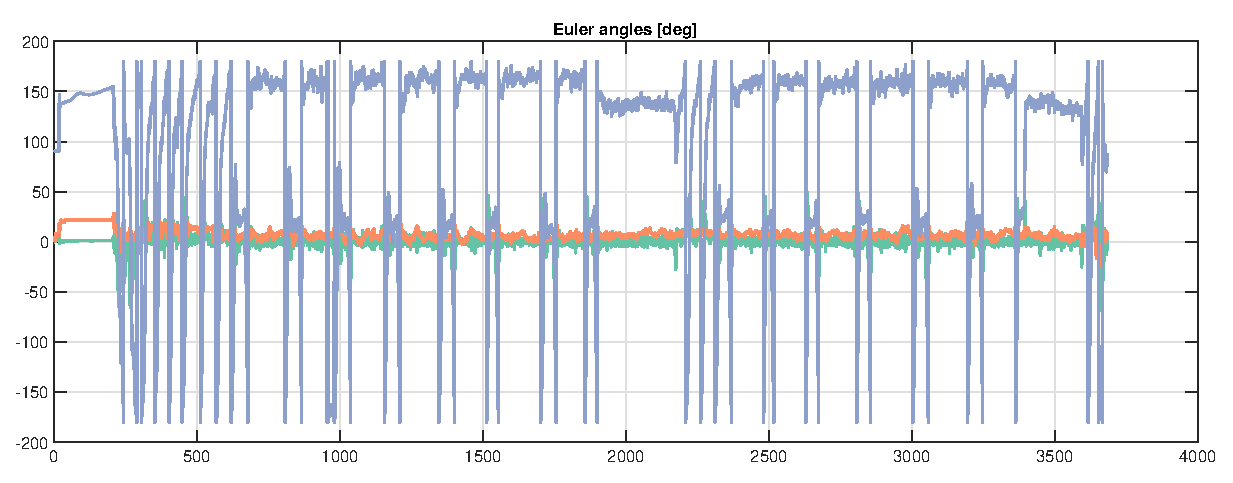
\includegraphics[width=0.8\linewidth]{figures/ga_2/real_bad_heading.eps}
    \caption{UAV estimated attitude without sensor error correction}
    \label{fig:ga_2_real_consistency}
\end{figure}

% discuss assumptions, linearity, convergence - knowing initial values? Robustness

One could argue that the benefits of the ESKF are twofold. Firstly, since the error dynamics are approximately linear, the optimality of the linear Kalman filter, which is lost when extending it to nonlinear process and measurement models with the EKF, are (approximately) retained. Secondly, since the IMU is treated as a control input and the IMU biases are estimated, we achieve robustness, as has previously been discussed. In the test implementations in this assignment, with both simulated and real data sets, this has been observed. By masking modelling errors, sensor errors, uncertainties and actual sensor biases within these states, the filter system is able to operate in a dynamic environment where the plant performs various different manoeuvres, even with wind disturbance and temperature fluctuations.

One could argue that the main limitation of the ESKF for inertial navigation is its slow convergence for deficient initial attitude values. In these tests of the filter, this has not been an issue, as good initial values were provided. One should note that this is not always the case. In many real-time applications, you cannot expect to turn on your INS and have good initial estimates of the attitude. If one tries to give an arbitrary attitude initialization to the ESKF, one observes poor estimates that are not at all usable. Due to length limitations this cannot be further explored here, but nevertheless this is a problem that could be further analysed and extensions to the ESKF could be added to handle this e.g. with optimization methods.
\section{Graded Assignment 3}\label{sec:graded_assignment_3}

% A full answer and result analysis is expected for task 3 and 4. For task 3 you should include a plot of the pose over time as well as the final estimated landmarks for your choice of parameters, in addition to NEES and NIS over time for the same set of parameters. In task 4 the same plots are expected, where the GPS can be used for ground truth. For both tasks it should be made clear why the parameters were chosen in terms of error metrics, consistency and overall result. Answers and analysis should connect theory and results to the real world, and show your understanding for the problem and solution. Try to connect the results on the simulated data to the results of the read data where and if it is possible. 

An extended Kalman filter was implemented for solving the SLAM problem in MATLAB. Specifically, the EKF-SLAM formulation in this report considers only the 2D case, with odometer measurements acting as control input. Furthermore, data association is done with the JCBB algorithm. For the relevant theory behind this EKF-SLAM formulation and JCBB, consult \cite[p. 185 - 196]{Edmund}.

\subsection{EKF-SLAM on simulated vehicle data set}

% Q, R, JCBB alphas
% NIS. Pose and lmks close to GT.

%The overall target was to minimize the difference between the estimated position and the ground truth, as well as decent NIS over time. Specifically we calculated the confidence interval over time with the size of the current innovation as the number of degrees of freedom. Initially, we set the noise covariance matrices higher than necessary, to get a rather conservative result, and decreased them as appropriatly. At the same time, we decreased the alphas used in the JCBB, as we could assume most of the measurements were from real landmarks. This resulted in a decently quick script, with the estimates being very close to the ground truth (with few / small offsets) and a decent NIS over time. 

The EKF-SLAM was first tuned using a simulated vehicle data set. The odometer measurement noise was tuned according to $Q = \text{diag}(\begin{array}{ccc}[(\sigma_u^2 & \sigma_v^2 & \sigma_\varphi^2 ]^{\top})\end{array}$, where $\sigma_u = \sigma_v = \SI{1e-1}{\meter\per\second}$ and $\sigma_\varphi = \SI{1e-2}{rad}$. The range-bearing measurement noise covariance was tuned according to $R = \text{diag}(\begin{array}{cc}[\sigma_r^2 & \sigma_\theta^2 ]^{\top})\end{array}$, where $\sigma_r = \SI{4e-2}{\meter}$ and $\sigma_\theta = \SI{2e-2}{rad}$. The JCBB algorithm was tuned by letting the individual compatability significance level be $\alpha_{ic} = \SI{1e-5}{}$ and the joint compatabiltiy significance level be $\alpha_{jc} = \SI{1e-10}{}$.

The system was tuned by trying to minimize the errors in pose and landmark estimates, while also looking at the calculated total NIS and NEES in pose. Note that in the NIS case the confidence interval was calculated at each time step, using the size of the current innovation as the number of degrees of freedom in the $\chi^2$ distribution. The estimated pose trajectory and landmark positions are presented in \cref{fig:ga_3_sim_trajectory}, and the consistency analysis plots are presented in \cref{fig:ga_3_sim_NIS}. We observe that 90\% of the NIS is inside the calculated the confidence interval, while 94.6\% of the NEES is inside the confidence intervals.

\begin{figure}[!htb]
    \centering
    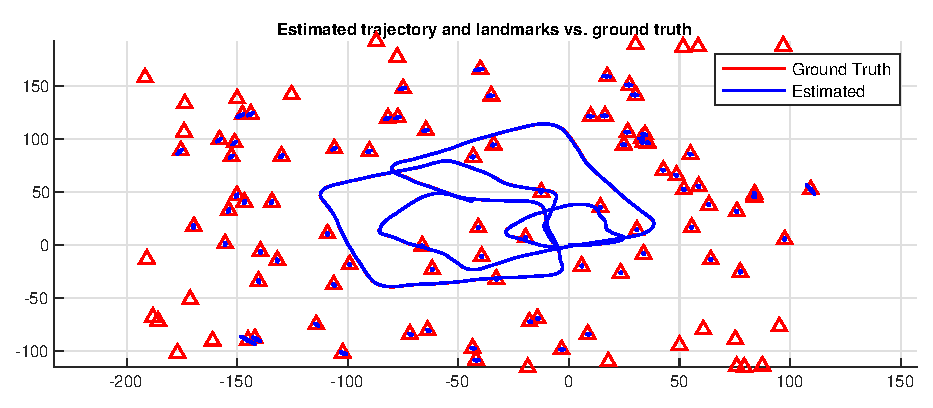
\includegraphics[width=0.6\linewidth]{figures/ga_3/sim_trajectory.eps}
    \caption{Estimated and ground truth pose trajectory and landmarks for simulated vehicle data}
    \label{fig:ga_3_sim_trajectory}
\end{figure}

\begin{figure}[!htb]
    \centering
    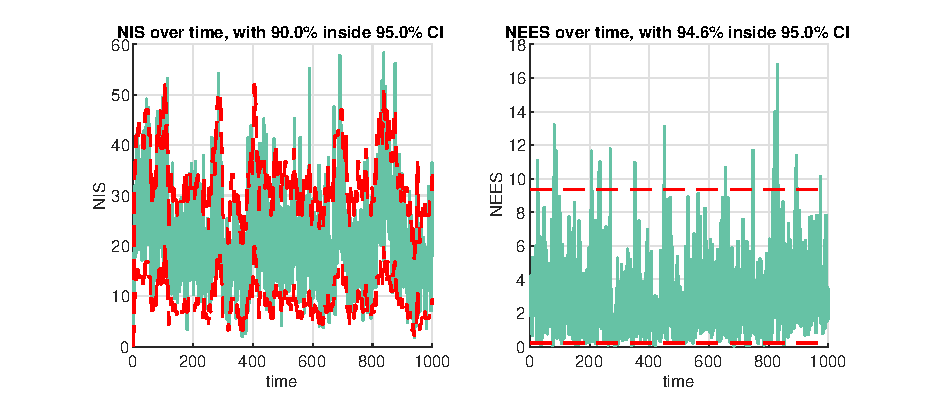
\includegraphics[width=0.8\linewidth]{figures/ga_3/sim_NIS.eps}
    \caption{Consistency for simulated vehicle data set with confidence intervals over time}
    \label{fig:ga_3_sim_NIS}
\end{figure}

Initially, the noise covariance matrices were set higher than necessary, to get a conservative result, and decreased until sufficient results were produced. At the same time, the compatibility alphas in the JCBB algorithm were reduced, as we could assume most of the measurements were from real landmarks.

% denseness, why?

%Discuss patterns in P - covariance. Discuss the two dots - why are these so high? They are not new states, but yet highly uncertain. It might just be the landmarks that are far away and that we have very few measurements off - might be the two landmarks with largest ellipses in trajectory plot? 
% Discuss using information matrix instead for speed? 

In \cref{fig:ga_3_sim_P} the covariance matrix and the inverse covariance matrix i.e. the information matrix at the last time step is presented. One should firstly note the denseness of the covariance matrix. This is a result of the fact that for the SLAM problem, all the states are highly correlated. We are trying to estimate the pose of the vehicle and the position of the landmarks relative to it simultaneously, which means that when we get additional information about the pose or a landmark from a measurement, we indirectly get information about all the other states as well. This means the covariance matrix will be very dense. Furthermore, we observe some additional structure in the covariance matrix, from the fact that landmarks that are close to each other will be more correlated than landmarks at different ends of the map. Finally, we also observe two outliers in the bottom right part of the diagonal. This might correspond to some of the landmarks in \cref{fig:ga_3_real_trajectory} with the largest covariance ellipses. These landmarks are far away from the trajectory of the vehicle and have therefore not been measured many times during the simulation. It then follows that they will be more uncertain than the rest and we get a few spikes in the covariance matrix.

Now consider the inverse of the covariance matrix i.e. the information matrix. When the covariance matrix is dense, the inverse matrix will naturally be sparse. As seen in \cref{fig:ga_3_sim_P} it is even approximately diagonal. This is a useful fact that could be used to reformulate the EKF equations in terms of the information matrix. This would be an interesting extension of the algorithm that might reduce computation time drastically. This reformulation is known in the literature as SEIF SLAM. 

\begin{figure}[!htb]
    \centering
    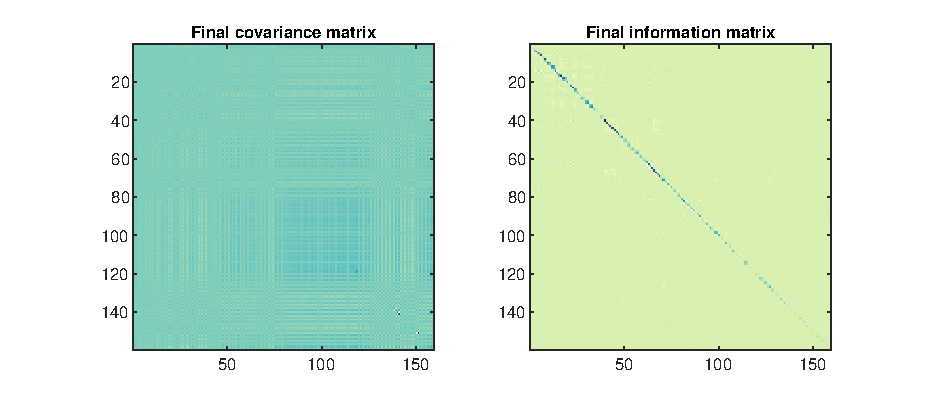
\includegraphics[width=0.7\linewidth]{figures/ga_3/sim_P.eps}
    \caption{Covariance matrix and information matrix for final timestep}
    \label{fig:ga_3_sim_P}
\end{figure}

% JCBB discussion

\subsection{EKF-SLAM on Victoria Park data set}

The EKF-SLAM code was then tested and tuned to the Victoria Park data set. The range-bearing measurement noise covariance was tuned with the same diagonal matrix, now with $\sigma_r = \SI{5e-2}{\meter}$ and $\sigma_\theta = \SI{5e-3}{rad}$. The odometer measurement noise covariance matrix was now tuned to be
\begin{equation}
    Q = \begin{bmatrix}
        0.25 & 0 & 0 \\
        0 & 0.25 & 0.0225 \\
        0 & 0.0225 & 0.0025 \\
    \end{bmatrix}.
\end{equation}
Notice how for this data set a high correlation between the measured sideways displacement $v$ and the measured heading $\varphi$. The JCBB individual and joint compatability significance levels were now tuned to be $\alpha_{ic} = \SI{1e-3}{}$ and $\alpha_{jc} = \SI{1e-3}{}$.

The system was largely tuned by the same process as for the simulated data, but there are several differences worth mentioning. Firstly, the pose ground truth is naturally no longer available, only GPS position measurements. This was plotted in relation to the estimated pose trajectory and landmarks, as seen in \cref{fig:ga_3_real_trajectory}. But there is no easy way to properly compare the estimate to the GPS measurement, as the EKF-SLAM algorithm only produces a local estimate in relation to how it was initialized. In \cref{fig:ga_3_real_trajectory} the GPS measurements were therefore rotated until the two different frames looked somewhat aligned.

\begin{figure}[!htb]
    \centering
    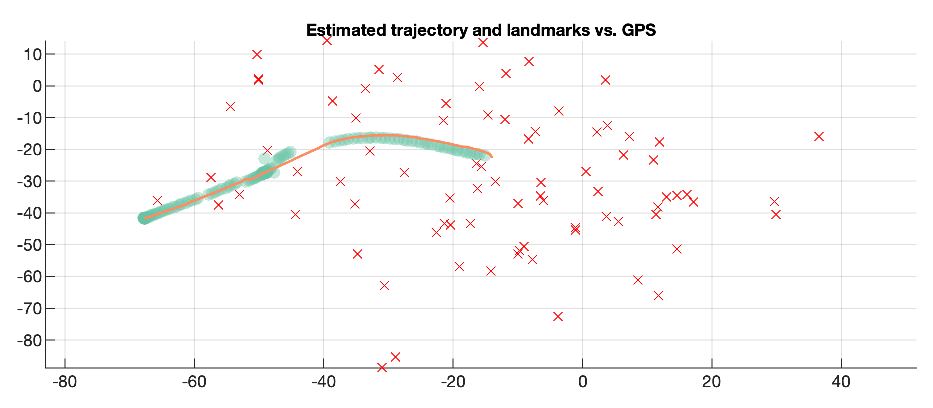
\includegraphics[width=0.6\linewidth]{figures/ga_3/real_trajectory.eps}
    \caption{Estimated pose trajectory, landmarks and GNSS measurements for Victoria Park data set}
    \label{fig:ga_3_real_trajectory}
\end{figure}

Since we no longer have the pose ground truth, the pose NEES is no longer available which also limits the available tools when tuning. But the NIS, again with a variable degree of freedom confidence interval, was actively used and is presented for the final tuning parameters in \cref{fig:ga_3_real_NIS}. It was calculated that 67\% of the NIS was inside the confidence intervals.  

\begin{figure}[!htb]
    \centering
    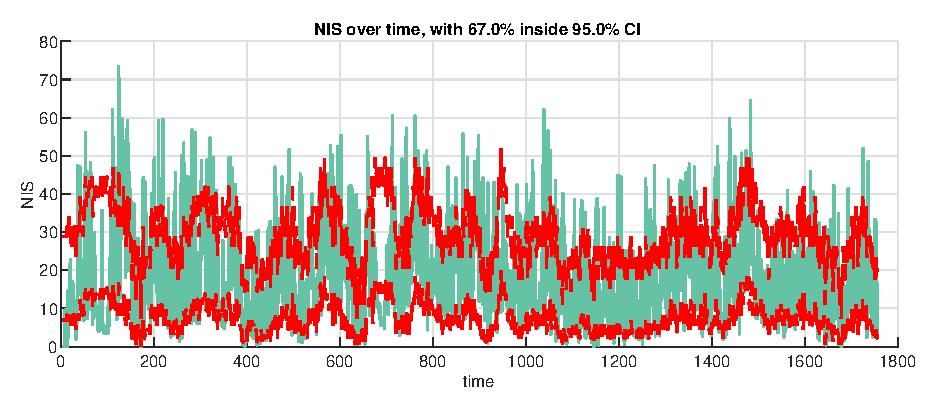
\includegraphics[width=0.7\linewidth]{figures/ga_3/real_NIS.eps}
    \caption{NIS for Victoria Park data set with confidence intervals over time}
    \label{fig:ga_3_real_NIS}
\end{figure}

One should also note the much higher compatibility alphas compared to the simulated data set. It was quickly observed while testing the system that the spread in range-bearing measurements of the landmarks was larger compared to the simulated case. It was concluded that the JCBB gating that was previously used was too low for this data set, and therefore increased. Another factor that influenced this tuning choice is the fact that each measurement that is not a part of the optimal choice with the most association matches from the JCBB algorithm are treated as new landmark states and added to the state vector. By increasing the individual and joint compatibility gate sizes we give JCBB more leeway, thereby reducing the number of new states added as the EKF-SLAM algorithm runs. Since, as previously discussed, the covariance matrix tends to be dense and very large, with a dimension in the hundreds, it is desirable to reduce the number of new states the algorithm adds to reduce computation time. It should be noted that JCBB will naturally use more time when the alphas are increased, as more association hypotheses must be considered. So how effective this strategy is in saving computation time is questionable, but this will slow down the growing state size which slows the algorithm down more and more over time, which was the primary concern here. 

% discuss EKF-SLAM assumptions.
% Discuss performance of EKF-SLAM. Why it sucks ass - fucked consistency and time scales with n^2 as we find more and more landmarks. Memory, quadratic scaling -> scales badly. Improvements, alternatives? Could decompose map into smaller independent maps? Robo-centric formulation? See book stuff. Different algorithms e.g. particle filter or graph-based approaches. 

When considering the performance of EKF-SLAM in these tests, one could argue that the performance is satisfactory, but several limitations are evident in the results. The first limitation, which applies to SLAM in general, is the fact that the estimated pose and landmark positions are only local estimates. While it is most important for the robot or vehicle to know its location relative to the environment, one can imagine several applications where global estimates are needed and this algorithm not being sufficient. One could remedy this by adding additional sensors to the system like a magnetometer, or simply making sure to initialize the system in the global frame. 

Another limitation is poor consistency, as a result of the fact that we are using an EKF. For the simulated data set the NEES did not evolve to be too large over time, but never the less it is a valid concern that the EKF will be too confident over time\cite{ekfslam}. One improvement to this is to formulate the EKF equations in a robocentric view. Alternatively, particle filter approaches or nonlinear observer theory can be used instead. 

Perhaps the more important limitation of EKF-SLAM is the memory and processing power requirements for the algorithm in large scale applications. Observe that the number of calculations and needed memory will scale quadratically for this algorithm. With the relatively small scale test using the Victoria Park data set, the script used about 10 minutes to finish $N=15000$ time steps, which corresponds to about 6,6 minutes of data, on a 2,7 GHz Intel Core i5. So for even this small scale example with only a few hundred landmarks the system was not able to operate in real-time. This demonstrates how infeasible it is to scale this algorithm to a more complex environment over a larger time horizon. For many applications, one can imagine that the number of landmarks could be several magnitudes larger than for this data set, and making it run online would not be feasible. This is not only because of the processing speed requirements but the memory requirements as well, when you have a dense covariance matrix consisting of millions of elements.

There are many possible improvements or alternatives that address these concerns. One idea is to simply separate the map into several independent parts to reduce the number of landmarks we are considering at the same time. This might allow us to better scale to a larger map. Reformulating the EKF-SLAM problem using the information matrix, as previously discussed, is also an alternative that could be explored. Graph-based methods are also based on the sparsity of the information matrix and could be used as an alternative to the EKF-SLAM. 


\section{Conclusion}\label{sec:conclusion}
In this report, several methods from the course TTK4250 - Sensor Fusion, and the results from applying them to different data sets, have been stated and discussed. The methods implemented were the tracking method \acrshort{imm_pdaf}, the inertial navigation method \acrshort{eskf} and the \acrshort{slam} method \acrshort{ekf_slam}. These methods have been tuned to give good results as well as consistency. By analysing the \acrshort{nis} and \acrshort{nees} where possible, 

% This does not have to be long, but try to write a few reasonable closing remarks.

% Quickly say what we have implemented and what results we got.

% Say how looking at errors and especially NIS and NEES was extensively used in all parts - shows the greatness of consistency analysis

% write some inspiring shit about how all this is applications of the almighty kalman filter. Especially how the trick with letting control input be a measurement is used in both ESKF and EKFSLAM. 


\addcontentsline{toc}{section}{Appendix} % Remove this if you don't want the appendix included in the table of contents.
\appendix

\section{MATLAB Code}\label{sec:matlab}
This section should contain your MATLAB code. DO NOT attach files posted online (that you didn't write). Note that the method used to input code below does not look as pretty when the lines are too long.

\subsection{plot\_constraint.m}\label{sec:plot_constraint_m}
\lstinputlisting{code/plot_constraint.m}\section{Simulink Diagrams}\label{sec:simulink}
This section should contain your Simulink diagrams. Just like the plots, these should be in vector format, like in \Cref{fig:simulink}. Make them tidy enough to understand.

\subsection{A Simulink Diagram}
\Cref{fig:simulink} shows a Simulink diagram. You can use the \texttt{print\_simulink.m} function, included in the source code repository for this document, to export a Simulink model to EPS\@.
\begin{figure}[htb]
	\centering
		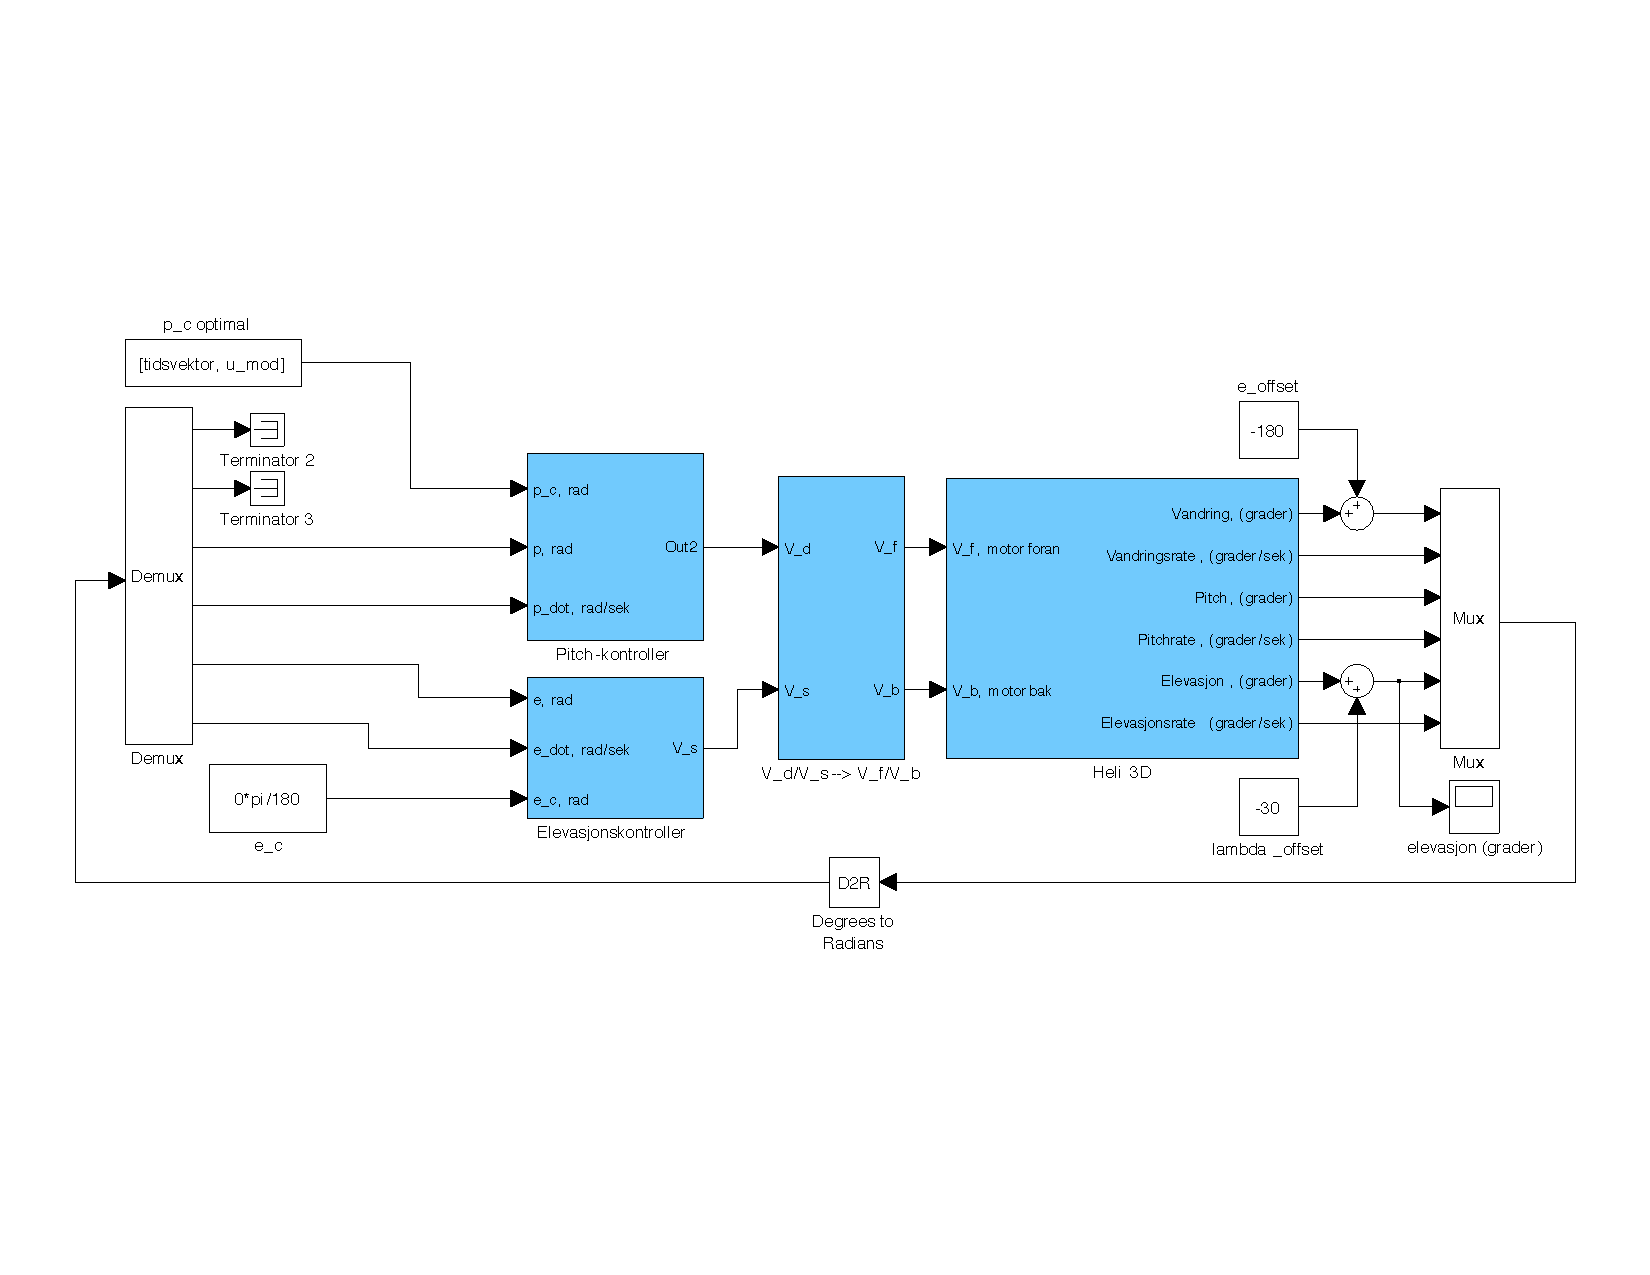
\includegraphics[width = \textwidth]{figures/simulink.pdf}
	\caption{A Simulink diagram.}
\label{fig:simulink}
\end{figure}

% \input simply inserts the contents of the file, while \include forces a \newpage.
% See \input vs. \include: http://tex.stackexchange.com/questions/246/when-should-i-use-input-vs-include

% References
\newpage
\addcontentsline{toc}{section}{References}
\printbibliography{}
\label{sec:bibliography}

\end{document}
